\input{formalia/preamble_udviklingsdokumentation}

\begin{document}
	
%Short TOC


\thispagestyle{empty}
\begin{flushright}
\vspace{3cm}

\phantom{hul}

\phantom{hul}

\phantom{hul}

\textsl{\Huge Remote Ischemic Conditioning} \\ \vspace{1cm}
\textsl{\Huge Udviklingsdokumentation} \\ \vspace{1cm}

\rule{\textwidth}{3mm} \\ \vspace{1.5cm}
\vspace{1cm}

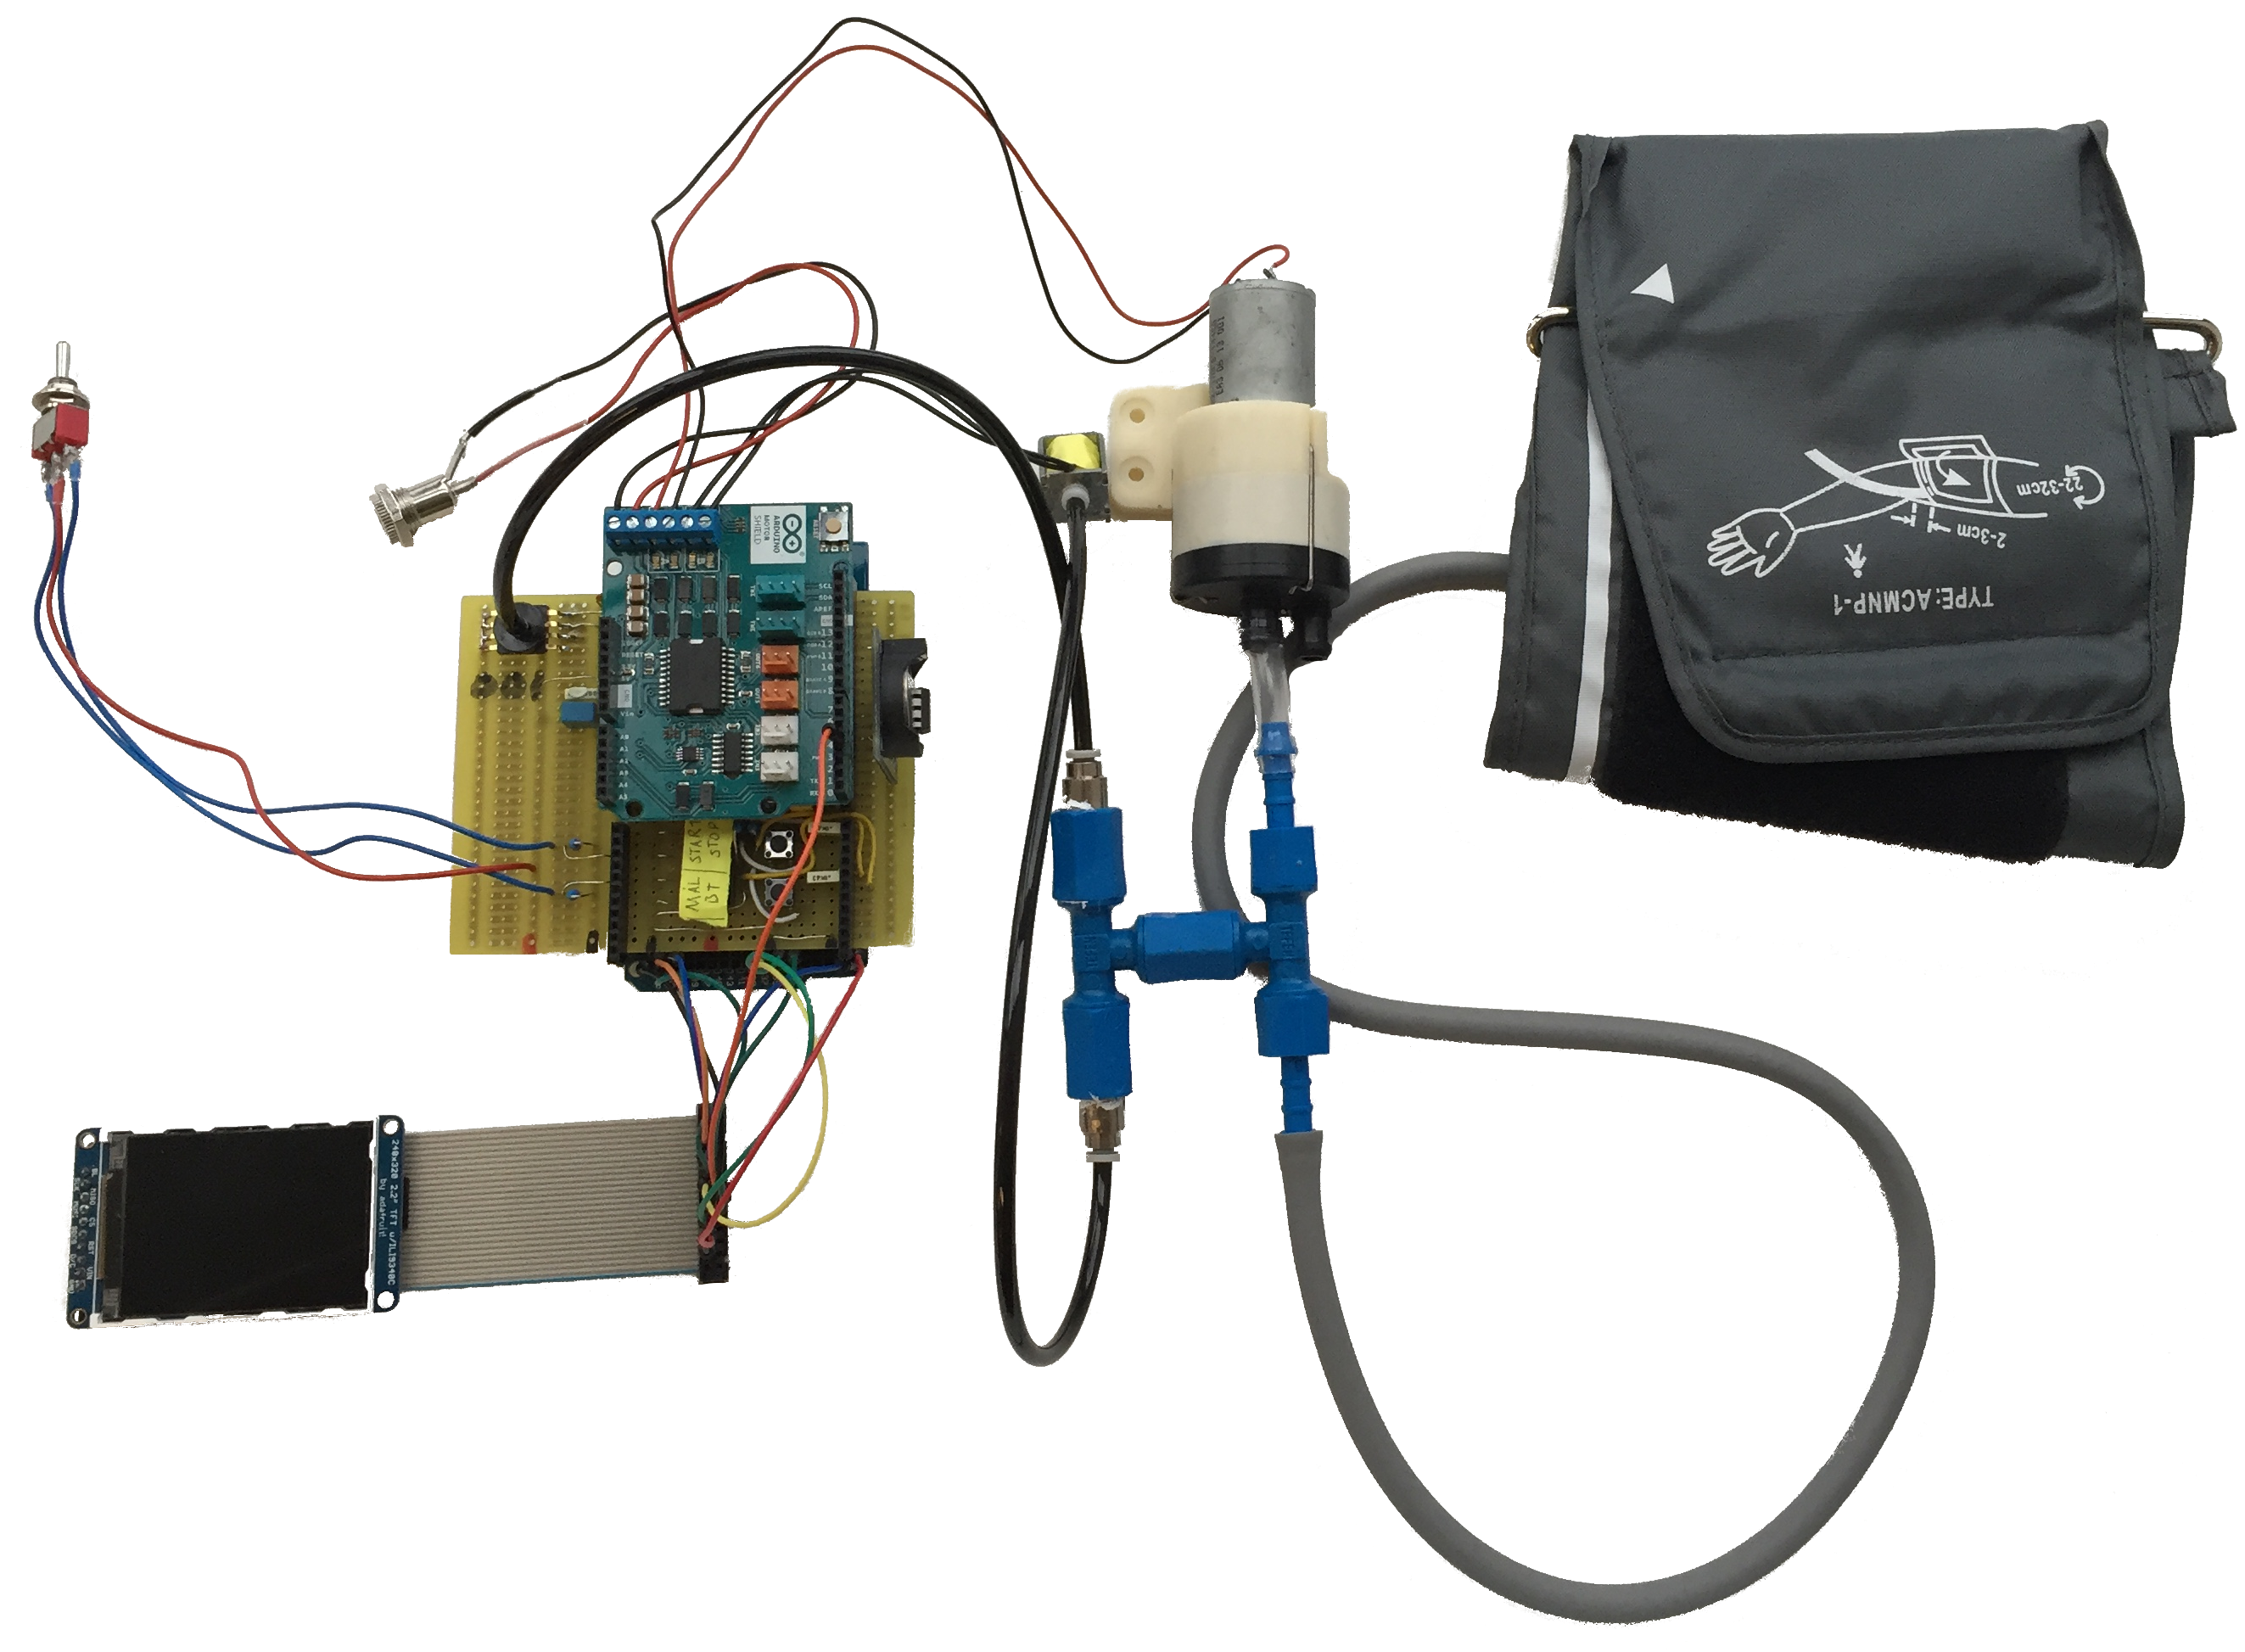
\includegraphics[width=0.9\textwidth]{formalia/forsidebillede.png}

\vspace{1cm} 
\textsc{\Large Bachelorprojekt \\
Gruppe 15155 \\
Karl-Johan Schmidt \\
Simon Vammen Grønbæk \\
Ingeniørhøjskolen, Aarhus Universitet \\
Efteråret 2015 \\}
\end{flushright}
	
% Dette er et titelblad designet til videregående uddannelser på et universitet
% Filen kræver:
% Universitetets logo:  AU-logo-DK eller AU-logo-DK
% Synopsis: En fil ved navn synopsis.tex

% Udarbejdet af: Jesper Nørgaard (jesper@noergaard.eu) 10. april 2012

\phantomsection
\pdfbookmark[0]{Titelblad}{titelblad}
\thispagestyle{empty}

\begin{minipage}[t]{0.48\textwidth}
\vspace*{-8pt}			

\includegraphics[height=2.5cm]{filer/AU-logo-DK}
\end{minipage}
\hfill
\begin{minipage}[t]{0.48\textwidth}
{\small 
\textbf{Ingeniørhøjskolen Aarhus}\\
Finlandsgade 22 \\
8200 Aarhus N \\
Tlf: 8715 0000 \\
http://www.ase.au.dk/}
\end{minipage}

\vspace*{1cm}

\begin{minipage}[t]{0.48\textwidth}
\textbf{Titel:} \\[5pt]\bigskip\hspace{2ex}
System design

\textbf{Projekt:} \\[5pt]\bigskip\hspace{2ex}
Remote Ischemic Conditioning

\textbf{Projektperiode:} \\[5pt]\bigskip\hspace{2ex}
Juli 2015 - December 2015

\textbf{Projektgruppe:} \\[5pt]\bigskip\hspace{2ex}
15155

\textbf{Deltagere:} \\[5pt]\hspace*{2ex}
Simon Vammen Grønbæk\\\hspace*{2ex}
Karl-Johan Schmidt \\\hspace*{2ex}


\textbf{Vejledere:} \\[5pt]\hspace*{2ex}
Peter Johansen \\\bigskip\hspace{2ex}

\textbf{Projektudbyder:} \\[5pt]\hspace*{2ex}
Rolf Blauenfeldt\\\bigskip\hspace{2ex}
\vspace*{4cm}

\textbf{Versionsnummer: 0.5} \\
\textbf{Sidetal: \pageref{lastPage}} \\
\textbf{Afsluttet 16-12-2015}

\end{minipage}
\hfill
\begin{minipage}[t]{0.483\textwidth}
	\textbf{Godkendelse:}\vspace{1cm}
\begin{table}[H]
	\centering
	\begin{tabular}{c}
		\underline{\phantom{mmmmmmmmmmmmmm}}  \\
		Karl-Johan Schmidt \vspace{2cm}\\
		\underline{\phantom{mmmmmmmmmmmmmm}} \\
		Simon Vammen Grønbæk \vspace{2cm}	\\
		\underline{\phantom{mmmmmmmmmmmmmm}} \\
		Peter Johansen \vspace{2cm}	\\
		\underline{\phantom{mmmmmmmmmmmmmm}} \\
		Rolf Blauenfeldt \vspace{2cm}	\\
	\end{tabular}
\end{table}
\end{minipage}

\vfill



\newpage

\startcontents[overall]
\printcontents[overall]{}{-1}{\chapter*{Indholdsfortegnelse}}
\newpage

\chapter*{Indledning}
\addcontentsline{toc}{chapter}{Indledning}
Udviklingsdokumentationen er en samling af skriftlige resultater igennem udviklingsfasen. Dokumentet samler kravspecifikationen, accepttesten, system designet og implementeringen i et fælles dokument. 

\section*{Formål}
Formålet med udviklingsdokumentationen er at beskrive udviklingsfasen og udarbejdelse af dokumentation, som beskriver produktet i hvert udviklingstrin. Et individuelt formål findes under hvert underdokument. 

\section*{Læsevejledning}
Dokumentet består af fire underdokumenter, hhv. kravspecifikation, accepttest, system design og implementering. En individuel læsevejledning findes under hvert underdokument. Hvert dokument har desuden sin egen indholdsfortegnelse. 


\part{Kravspecifikation} \label{part:ks}
\stopcontents[overall]
\startcontents[ks]
\documentclass[11pt]{article}
\usepackage[utf8]{inputenc}  % To control and create table of content
\usepackage{fancyhdr} 	% To create header
\usepackage{dirtytalk} % To create citations
\usepackage{array} % To control and create fixed size tables
\usepackage{longtable}
\usepackage{graphicx}
\graphicspath{ {Illustrationer/} }

\pagestyle{fancy}
\fancyhf{}
\lhead{Kravspecifikation}
\rhead{Version 0.1}
\rfoot{Page \thepage}

\renewcommand*\contentsname{Indholdsfortegnelse}

\begin{document}
	\begin{titlepage}
		\begin{center}
			\Large\textbf{Kravspecifikation}\\
			\large\textit{Version: 0.1}
		\end{center}
	\end{titlepage}
	
	\tableofcontents
	\newpage
	
	\section{Introduktion og baggrund}
	Formålet med dette dokument er at beskrive funktionelle og ikke-funktionelle krav for per konditionerings blodtryks apparatet. De funktionelle krav vil blive beskrevet ved hjælp af fully dressed use case diagrammer. 
	
	Beskrivelse af projektet: 
	
	\say{\textit{Akut blodprop i hjernen (Acute Ischemic Stroke – AIS) er en førende årsag til død og alvorlig handicap hos personer over 60 år.Intravenøs trombolysebehandling administreret indenfor 4,5 time fra symptomdebut er den nuværende bedste medicinske behandling. Grundet sikkerhedshensyn og det snævre tidsvindue er det desværre kun et fåtal af AIS patienterne, der modtager denne behandling. Målet er at opløse blodproppen og genoprette blodforsyning og dermed redde hjernevæv, der lider af iltmangel men endnu ikke er dødt. Om et område af hjernen dør eller står til at redde ved en blodprop afhænger ikke kun af selve blodproppen men også om hjernen er i stand til at få blod via omveje dannet af hjernens små blodkar. Et område af hjernen går til grunde med det samme (infarktkernen). Denne kerne af dødt hjernevæv kan i dagene efter en blodprop sprede sig og vokse. Der er således behov for at kunne beskytte hjernen mod iltmangel og øge andelen af hjernevæv, der overlever en blodprop. Iltmangel induceret periodevis i et fjernt organ (remote ischemic conditioning RIC) kan udføres ved at puste en blodtryksmanchet med afklemning af armen. Konditionering kan leveres som pre, per, og postconditionering, afhængig af om stimulus udøves før iltmangel, under iltmangel men før blodproppen er opløst og endelig efter blodproppen er opløst. Dyrestudier og senest kliniske studier har vist at RIC kan mindske det område af hjertet eller hjernen, der dør ved en blodprop. Det er ikke tilstrækkeligt undersøgt om RIC mindsker risikoen for handicap efter en blodprop i hjernen.}}
	
	\section{System beskrivelse}
	System er beregnet til behandling af patienter med \textit{acute ischemic stroke(AIS)}. Formålet er pre, per og postkonditioning af disse patienter. Systemet skal kunne lave arteriel okklusion i de øverste ydre ekstremiteter. For at sikre tilstrækkelig okklusion, skal det systoliske blodtryk først måles og derefter pumpe cuffen op til plus 25 mmHg over det målet tryk. Som minimum skal der afklemmes med et tryk på 180 mmHg. Okklusionen bliver holdt konstant i 5 minutter, hvor efter trykket lukkes ud der holdes en "pause" på 5 minutter. Denne process gentages ind til konditioneringen er færdig. 

	\section{Funktionelle krav}
	
	%Aktør beskrivelse
		\subsection{Aktør beskrivelse}
	\begin{center}
		\begin{tabular}{ | m{4cm} | m{8cm}| } 
			\hline
			Aktørnavn& Patient \\ 
			\hline
			Aktørtype & Primær og sekundær \\ 
			\hline
			Beskrivelse af aktør & En person med AIS som skal konditioneres\\ 
			\hline
		\end{tabular}
	\end{center}
	
	\begin{center}
		\begin{tabular}{ | m{4cm} | m{8cm}| } 
			\hline
			Aktørnavn& Medicinsk personale / Bruger \\ 
			\hline
			Aktørtype & Primær og sekundær \\ 
			\hline
			Beskrivelse af aktør & Aktør som påmontere cuff og styre konditionering eller person som observere de gemte data fra behandlingsforløb\\ 
			\hline
		\end{tabular}
	\end{center}
	
	\begin{center}
		\begin{tabular}{ | m{4cm} | m{8cm}| } 
			\hline
			Aktørnavn& Database \\ 
			\hline
			Aktørtype & Sekundær \\ 
			\hline
			Beskrivelse af aktør & Gemmer data og logs information omkring konditionerings forløb\\ 
			\hline
		\end{tabular}
	\end{center}
	
	\begin{center}
		\begin{tabular}{ | m{4cm} | m{8cm}| } 
			\hline
			Aktørnavn& Bruger \\ 
			\hline
			Aktørtype & Primær \\ 
			\hline
			Beskrivelse af aktør & Person der gør brug af konditioneringsapparatet til okklusionstræning, denne person behøver ikke besidde særlig faglig viden \\ 
			\hline
		\end{tabular}
	\end{center}
	\pagebreak
	
	%Use case 1
	\subsection{Use case 1 - Konditionering}
\begin{center}
		\begin{longtable}{ | p{0.24\textwidth} | p{0.7\textwidth}| } 
			\hline
			Mål & Gennemføre én konditioneringsbehandling  \\ 
			\hline
			Initiering &  Medicinsk personale\\
			\hline
			Aktører og interessenter & 
			\begin{itemize}
				\item Medicinsk personale(primær)
				\item Patient (sekundær)
			\end{itemize} \\ 
			\hline
			Referencer & Use case 3 \\ 
			\hline
			Antal samtlige forekomster & En til mange\\ 
			\hline	
			Startbetingelser & 
			\begin{itemize}
				\item Mode switch er sat til “\textit{Konditionering}”
			\end{itemize} \\ 
			\hline
			Slutbetingelser & 
			\begin{itemize}
				\item \textit{Antal cyklusser} er gennemført og gemt på hukommelsen
			\end{itemize} \\ 
			\hline
			Normal forløb & \begin{enumerate}
				\setlength\itemsep{0cm} % Decrease line distance
				\item \textit{Medicinsk personale} placerer manchetten på patienten
				\item \textit{Medicinsk personale} trykker på knappen [Start/Stop]
				\item Et nyt patient ID genereres
				\subitem[Undtagelse \#1] 
				\item Patient ID’et vises på skærmen
				\item Blodtrykket måles via \textit{use case 3}
				\subitem[Undtagelse \#2]
				\item Blodtrykket vises på displayet og værdien gemmes i hukommelsen
				\item Manchetten fyldes med luft til et tryk på 25 mmHG over systolisk tryk (minimum 200 mmHg)					
				\item Tidsstempel gemmes når trykket er opnået
				\item Trykket opretholdes i 5 minutter(Okklusion) og resterende tid vises på displayet
				\item Deflaterer manchetten helt og forbliver i dette stadie i 5 min(Reperfusion) Ved deflation start gemmes tidsstempel. Tid til næste okklusion vises på displayet
				\item Gentag punkt 7-10 (en \textit{cyklus}) fire gange. Det nuværende cyklus nummer vises i displayet
			\end{enumerate} \\ 
			\hline
			Undtagelser & [Undtagelse \#1] Et patient ID eksisterer allerede på apparatet. Der genereres ikke noget nyt patient ID.
			
			[Undtagelse \#2] Blodtrykket kunne ikke måles. Gentag use case 3 hvis undtagelse 2 ikke lige er eksekveret. Ellers skrives i display “FEJL kunne ikke måle blodtryk” og use casen stopper  \\
			\hline
			\caption{\textit{Fully dressed} use case diagram over use case 1}
		\end{longtable}
		
	\end{center}
	
	%Use case 2
		\subsection{Use case 2 - Initialiser blodtryksmåling }
	Denne use case beskriver hvordan en blodtryksmåling initieres. Use casen er gældende når en blodtryksmåling skal foretages uden af apparatet udfører konditioneringsbehandling, (Se tabel \ref{tab:uc2}).
	\begin{table}[H]
		\begin{center}
			\begin{tabular}{ | p{0.24\textwidth} | p{0.7\textwidth}| } 
				\hline
				Mål& Mål et blodtryk\\ 
				\hline
				Initiering &  Medicinsk personale\\
				\hline
				Aktører og interessenter & 
				\begin{itemize}
					\item Medicinsk personale(primær)
					\item Patient (sekundær)
				\end{itemize} \\ 
				\hline
				Referencer & Mål blodtryk(UC3) \ref{title:uc3} \\ 
				\hline
				Antal samtlige forekomster & Ingen\\ 
				\hline	
				Startbetingelser & 
				\begin{itemize}
					\item Manchetten er placeret på armen
					\item Mode switch er sat til “\textit{Konditionering}”
				\end{itemize} \\ 
				\hline
				Slutbetingelser & 
				\begin{itemize}
					\item Patientens blodtryk er målt
				\end{itemize} \\ 
				\hline
				Normal forløb & \begin{enumerate}
					\setlength\itemsep{0cm} % Decrease line distance
					\item Brugeren trykker på [Mål blodtryk]
					\subitem [Undtagelse \#1]
					\item Et nyt patient ID genereres
					\subitem [Undtagelse \#2] 
					\item Patient ID’et vises på skærmen
					\item Blodtrykket måles via \textit{use case 3} (Se \ref{title:uc3})
					
				\end{enumerate} \\ 
				\hline
				Undtagelser & [Undtagelse \#1] SD kortet er ikke monteret korrekt
				
				[Undtagelse \#2] Et patient ID eksisterer allerede på apparatet. Der genereres ikke noget nyt patient ID. \\ 
				\hline
				
			\end{tabular}
		\end{center}
		\caption{\textit{Fully dressed} use case diagram over use case 2} \label{tab:uc2}
			\end{table}
		\newpage
	
	%Use case 3
		\subsection{Use case 3 - Mål blodtryk}
		\begin{center}
			\begin{tabular}{ | m{4cm} | m{8cm}| } 
				\hline
				Goal& Mål et systolisk, diastolisk og middel(MAP) tryk\\ 
				\hline
				Initiation &  Use case 1 eller 2\\
				\hline
				Actors and stakeholders & - \\
				\hline
				References & - \\ 
				\hline
				Number of concurrent occurrences & En til mange\\ 
				\hline	
				Precondition & 
				\begin{itemize}
					\item Patient ID er oprettet
					\item Manchetten er placeret på armen
					\item Mode switch er sat til “\textit{Konditionering}”
				\end{itemize} \\ 
				\hline
				Postcondition & 
				\begin{itemize}
					\item Blodtrykket er mål
				\end{itemize} \\ 
				\hline
				Main scenario & \begin{enumerate}
					\setlength\itemsep{0cm} % Decrease line distance
					\item Manchetten fyldes til tryk over systolisk niveau 
					\item Luften lukkes gradvist ud og det systoliske tryk registreres 
					\item Middel trykket (MAP) måles 
					\item Det diastoliske tryk udregnes ud fra systole og MAP 
					\item Blodtrykket vises på skærmen og værdien gemmes i hukommelsen med et tidsstempel 
				\end{enumerate} \\ 
				\hline
				Extensions & -\\ 
				\hline
			\end{tabular}
		\end{center}
			\pagebreak
	
	%Use case 4
		\subsection{Use case 4 - Overfør data}
	I tabel \ref{tab:uc4} beskrives forløbet når data skal eksporteres fra \textit{Konditioneringsapparatet}. Denne use case sikre at SD kortet håndteres ens hver gang data eksportes og dette mindsker fejl. 
	\begin{table}[H]
		\begin{center}
			\begin{tabular}{ | p{0.24\textwidth} | p{0.7\textwidth}| } 
				\hline
				Mål & Eksportér data fra blodtryksapparat til databasen\\ 
				\hline
				Initiering &  Medicinsk personale\\
				\hline
				Aktører og interessenter & 
				\begin{itemize}
					\item Medicinsk personale(primær)
					\item Patient (sekundær)
				\end{itemize} \\ 
				\hline
				Referencer & - \\ 
				\hline
				Antal samtlige forekomster & Én pr behandlingsforløb \\ 
				\hline	
				Startbetingelser & 
				\begin{itemize}
					\item Der eksisterer en logfil på hukommelsen
				\end{itemize} \\ 
				\hline
				Slutbetingelser & 
				\begin{itemize}
					\item Logfilen er overført til database
					\item Blodtryksapparat udstyres med formateret hukommelse og klar til næste patient
				\end{itemize} \\ 
				\hline
				Normal forløb & \begin{enumerate}
					\setlength\itemsep{0cm} % Decrease line distance
					\item Tag SD kortet ud af blodtryksapparatet 
					\item Sæt SD kortet i computeren og overfør filen 
					\item Formatér SD kortet
					\item Sæt SD kortet tilbage i konditioneringsapparatet 
				\end{enumerate} \\ 
				\hline
				Undtagelser & -\\ 
				\hline
			\end{tabular}
		\end{center}
		
			\caption{\textit{Fully dressed} use case diagram over use case 4} \label{tab:uc4}
		\end{table}
			\newpage
	
	%UseCase 5
		\subsection{Use case 5 - Sikkerhedskontrol med pulsoximeter}
	Denne use case viser hvordan \textit{Konditioneringsapparatet} skal håndtere sikkerhedskontrol under et konditioneringsforløb, (Se tabel \ref{tab:uc5}).
	\begin{table}[H]
		\begin{center}
			\begin{tabular}{ | p{0.24\textwidth} | p{0.7\textwidth}| } 
				\hline
				Mål & Sikre at patientens kredsløb tåler konditionering \\ 
				\hline
				Initiering &  Konditionering (UC1)\\
				\hline
				Aktører og interessenter & 
				\begin{itemize}
					\item Patient (sekundær)
				\end{itemize} \\ 
				\hline
				Referencer & - \\ 
				\hline
				Antal samtlige forekomster & Ingen \\ 
				\hline	
				Startbetingelser & 
				\begin{itemize}
					\item Konditionering (UC1) (Se \ref{title:uc1}) igangværende
					\item Pulsoximeteret er monteret på patients finger
					\item Patient har gennemført én afklemnings cyklus
 				\end{itemize} \\ 
				\hline
				Slutbetingelser & 
				\begin{itemize}
					\item Patients tilstand er bestemt 
				\end{itemize} \\ 
				\hline
				Normal forløb & \begin{enumerate}
					\setlength\itemsep{0cm} % Decrease line distance
					\item Saturation detekteres
					\item Saturation gemmes på SD-kort
					\item Saturation er tilfredsstillende
					\subitem [Undtagelse \#1.1][Undtagelse \#1.2]
					\item Behandlingen kan fortsætte
				\end{enumerate} \\ 
				\hline
				Undtagelser &  [Undtagelse \#1.1] Tegn på dårlig kredsløb: Blodtryksapparatet stopper konditionerings forløbet 
				[Undtagelse \#1.2] Kør use case 7\\ 
				\hline
			\end{tabular}
		\end{center}
		\caption{\textit{Fully dressed} use case diagram over use case 5} \label{tab:uc5}
	\end{table}
			\newpage
	
	%UseCase 6
		\subsection{Use case 6 - Sikkerhedskontrol med pulsoximeter}
		\begin{center}
			\begin{tabular}{ | m{4cm} | m{8cm}| } 
				\hline
				Goal& Gennemføre okklusion af venøs kredsløb under træning  \\ 
				\hline
				Initiation &  Bruger\\
				\hline
				Actors and stakeholders & 
				\begin{itemize}
					\item Bruger (primær)
				\end{itemize} \\ 
				\hline
				References & - \\ 
				\hline
				Number of concurrent occurrences & En pr træningspas \\ 
				\hline	
				Precondition & 
				\begin{itemize}
					\item Mode switch er sat til  “\textit{okklusionstræning}”
 				\end{itemize} \\ 
				\hline
				Postcondition & 
				\begin{itemize}
					\item Okklusions træningssæt gennemført
				\end{itemize} \\ 
				\hline
				Main scenario & \begin{enumerate}
					\setlength\itemsep{0cm} % Decrease line distance
					\item Montere manchetten på arm/ben
					\item Tryk på knap [Start/Stop]
					\item Manchetten pumpes op til 100mmHg
					\item Træningssættet begyndes og trykkes holdes konstant på 100mmHg (+/-10mmHg)
					\item Tryk på knap [Stop]
					\item Manchetten deflateres
				\end{enumerate} \\ 
				\hline
				Extensions & - \\ 
				\hline
			\end{tabular}
		\end{center}
	\pagebreak
		
	
	%UseCase 7
		\subsection{Use case 7 - Afbryd}
	Når et givet scenarie skal afbrydes udføres use case 7. Denne use case (Se tabel \ref{tab:uc7}) sikre at \textit{Konditioneringsapparatet} kan afbrydes når som helst og sørge for at manchetten tømmes for luft. 
	\begin{table}[H]
			\begin{center}
			\begin{tabular}{ | p{0.24\textwidth} | p{0.7\textwidth}| } 
				\hline
				Mål & Tømme manchetten for luft og afbryde nuværende procedure \\ 
				\hline
				Initiering &  Medicinsk personale, Patient\\
				\hline
				Aktører og interessenter & 
				\begin{itemize}
					\item Medicinsk personale 
					\item Bruger 
				\end{itemize} \\ 
				\hline
				Referencer & Konditionering (UC1)(Se \ref{title:uc1}), Mål blodtryk (UC3)(Se \ref{title:uc3}) og Okklusionstræning (UC6)(Se \ref{title:uc6}) \\ 
				\hline
				Antal samtlige forekomster & En til mange \\ 
				\hline	
				Startbetingelser & 
				\begin{itemize}
					\item Konditionering (UC1) eller Okklusionstræning (UC6) er igangværende				\end{itemize} \\ 
				\hline
				Slutbetingelser & 
				\begin{itemize}
					\item Behandlingen er afbrudt og manchetten er tom for luft
				\end{itemize} \\ 
				\hline
				Normal forløb & \begin{enumerate}
					\setlength\itemsep{0cm} % Decrease line distance
					\item Brugeren trykker på knappen [Start/Stop konditionering]
					\item Den igangværende use case afbrydes
					\item Manchetten tømmes for luft og tidsstempel med “\textit{Afklemning afbrudt} = false(0)” gemmes i hukommelsen
					\subitem[Undtagelse \#1]
				\end{enumerate} \\ 
				\hline
				Undtagelser & [Undtagelse \#1] Use case 6 er aktiv: ingen data gemmes i hukommelsen. \\ 
				\hline
			\end{tabular}
		\end{center}
			\caption{\textit{Fully dressed} use case diagram over use case 7} \label{tab:uc7}
		\end{table}
	\newpage

		
	
	%UseCase8
		\subsection{Use case 8 - Setup}
	Use case 8 (Se tabel \ref{tab:uc8}) beskriver forløbet når der skal ændrings i konditioneringsprotokollen. Her kan ændres i tiden pr cyklus og antallet af cyklusser. 
		\begin{table}[H]
				\begin{center}
			\begin{tabular}{ | p{0.24\textwidth} | p{0.7\textwidth}| } 
				\hline
				Mål & Ændre konditioneringsforholdene \\ 
				\hline
				Initiation &  Medicinsk personale\\
				\hline
				Aktører og interessenter & 
				\begin{itemize}
					\item Medicinsk personale 
				\end{itemize} \\ 
				\hline
				Referencer & Illustration over setup \\ 
				\hline
				Antal samtlige forekomster & En til mange \\ 
				\hline	
				Startbetingelser & 
				\begin{itemize}
					\item Mode switch er sat til “\textit{setup}” 
					\item Displayet er ændret til setup
 				\end{itemize} \\ 
				\hline
				Slutbetinglser & 
				\begin{itemize}
					\item Cyklus længden og/eller antallet er cyklusser er ændret
				\end{itemize} \\ 
				\hline
				Normal forløb & \begin{enumerate}
					\setlength\itemsep{0cm} % Decrease line distance
					\item Brugeren trykker på knappen [Mål blodtryk]  for at vælge \textit{Tid pr cyklus}
					\item Bruger trykker på knappen [Start/Stop] for at ændre \textit{Tid pr cyklus}
					\item Bruger trykker på knappen [Mål blodtryk]  for at gemme ændringen
					\item Bruger trykker på knappen [Start/Stop] for at navigere til \textit{Antal cyklusser}
					\item Ved knap tryk på [Mål blodtryk]  vælges \textit{Antal cyklusser}
					\item Ved knap tryk på [Start/Stop] ændre \textit{Antal cyklusser}
					\item Brugeren trykker på knappen [Mål blodtryk] for at gemme ændringen
				\end{enumerate} \\ 
				\hline
				Undtagelser & -  \\ 
				\hline
			\end{tabular}
		\end{center}

			\caption{\textit{Fully dressed} use case diagram over use case 8} \label{tab:uc8}
		\end{table}
			\newpage

	
	\section{Ikke-funktionelle krav }
	
	\subsection{Filformat og opsætning}
	\begin{enumerate}
		\setlength\itemsep{0cm} % Decrease line distance
		\item Data logged i formatet .csv og hver kolonne indeholder følgende værdier og enheder: 
		\begin{enumerate}
			\item Tidsstempel [yy:mm:dd hh:mm:ss]
			\item Afklemningstryk [mmHg]
			\item Gennemført afklemning [Boolean]
			\item Systoliske blodtryk [mmHg]
			\item Middelblodtryk (MAP) [mmHg]
			\item Diastolisk blodtryk [mmHg]
		\end{enumerate}
		\item Der oprettet én fil pr patient, med filnavn tilsvarende det unikke patient ID
	\end{enumerate}
	
	\subsection{Patient ID}
	\begin{enumerate}
		\setlength\itemsep{0cm} % Decrease line distance
		\item Består af karaktererne A-Z og tallene 0-9
		\begin{enumerate}
			\item ID’et er fem karakterer lang: ***** svarende til 60 millioner kombinationer
			\item ID’et er ikke case sensitiv
		\end{enumerate}
	\end{enumerate}
	
	
	\subsection{Hukommelse}
	\begin{enumerate}
		\setlength\itemsep{0cm} % Decrease line distance
		\item Information lagres på micro SDSC af typen:
		\begin{enumerate}
			\item Class 4
			\item Fil system [fat32] og minimum 128mb
		\end{enumerate}
	\end{enumerate}
	
	\subsection{Forsyning}
	\begin{enumerate}
		\setlength\itemsep{0cm} % Decrease line distance
		\item Konditionerings apparatet skal forsynes med 12V, min 2A
		\begin{enumerate}
			\item DC-connector (angiv diameter) 
			\item 8 stk AAA batterier (1,5V)
		\end{enumerate}
	\end{enumerate}
	
	%User interface 
	\chapter{User interface}
User interface består overordnede af en skærm og 2 knapper. En knap til at start og stoppe funktioner og en knap til at måle blodtryk. Til brugerfeedback er der en display hvorpå trykket, patient ID, resterende tid og antallet af gennemførte cyklusser vises. Apparatet betjenes i tre forskellige stadier “Konditionering, Okklusion og setup”. Disse tre stadier er beskrevet med hver siden illustration nedenfor. For at skifte mellem disse stadier er der en mode switch på bagsiden af apparatet, den er også beskrevet nedenfor: 

\section{Konditionering}
\begin{figure}[H]
	\includegraphics[width=\textwidth]{Kravspecifikation/Illustrationer/KonditioneringGUI}
	\caption{Illustration over brugergrænseflade ved konditionering}
\end{figure}

\section{Okklusion}
\begin{figure}[H]
	\includegraphics[width=\textwidth]{Kravspecifikation/Illustrationer/OkklusionGUI}	
	\caption{Illustration over brugergrænseflade ved okklusion}
\end{figure}


\section{Setup}
\begin{figure}[H]
	\includegraphics[width=\textwidth]{Kravspecifikation/Illustrationer/SetupGUI}
	\caption{Illustration over brugergrænseflade ved setup}
\end{figure}


\section{Bagside}
\begin{figure}[H]
	\includegraphics[width=\textwidth]{Kravspecifikation/Illustrationer/BagsideGUI}	
	\caption{Illustration over brugergrænseflade på bagsiden af \textit{Konditioneringsapparatet} }
\end{figure}

\label{lastPage}

	
	
\end{document}
\stopcontents[ks]
\resumecontents[overall]
\newpage

\part{Accepttest} \label{part:at}
\stopcontents[overall]
\startcontents[at]
\documentclass[11pt]{article}
\usepackage[utf8]{inputenc}  % To control and create table of content
\usepackage{fancyhdr} 	% To create header
\usepackage{dirtytalk} % To create citations
\usepackage{array} % To control and create fixed size tables
\usepackage{longtable}
\usepackage{graphicx}
\usepackage{enumitem}
\graphicspath{ {Illustrationer/} }

\pagestyle{fancy}
\fancyhf{}
\lhead{Kravspecifikation}
\rhead{Version 0.1}
\rfoot{Page \thepage}

\renewcommand*\contentsname{Indholdsfortegnelse}

\begin{document}
	\begin{titlepage}
		\begin{center}
			\Large\textbf{Accepttest}\\
			\large\textit{Version: 0.1}
		\end{center}
	\end{titlepage}
	
	\tableofcontents
	\newpage
	
	\section{Funktionelle krav}
	
		\begin{center}
			\begin{tabular}{ | m{3cm} | m{3cm}| m{3cm}| m{3cm}| }
			\hline
			Krav nr.: & Forventet resultat & Test metode & Resultat  \\
			\hline
			\paragraph{hej}  &  &  &   \\
			\hline
			&  &  &  \\
			\hline
			&  &  &  \\
			\hline
			&  &  &   \\
			\hline
			&  &  &  \\
			\hline
			&  &  &  \\
			\hline
			&  &  &   \\
			\hline
			&  &  &  \\
			\hline
			&  &  &  \\
			\hline
		\end{tabular}
		\end{center}

	
	\end{document}
\stopcontents[at]
\resumecontents[overall]
\newpage

\part{ System design} \label{part:sd}
\stopcontents[overall]
\startcontents[sd]
\input{filer/preamble_SystemArk}

\begin{document}
	
	
	%Frontpage
	\thispagestyle{empty}
\begin{flushright}
\vspace{3cm}

\phantom{hul}

\phantom{hul}

\phantom{hul}

\textsl{\Huge Remote Ischemic Conditioning} \\ \vspace{1cm}
\textsl{\Huge Udviklingsdokumentation} \\ \vspace{1cm}

\rule{\textwidth}{3mm} \\ \vspace{1.5cm}
\vspace{1cm}

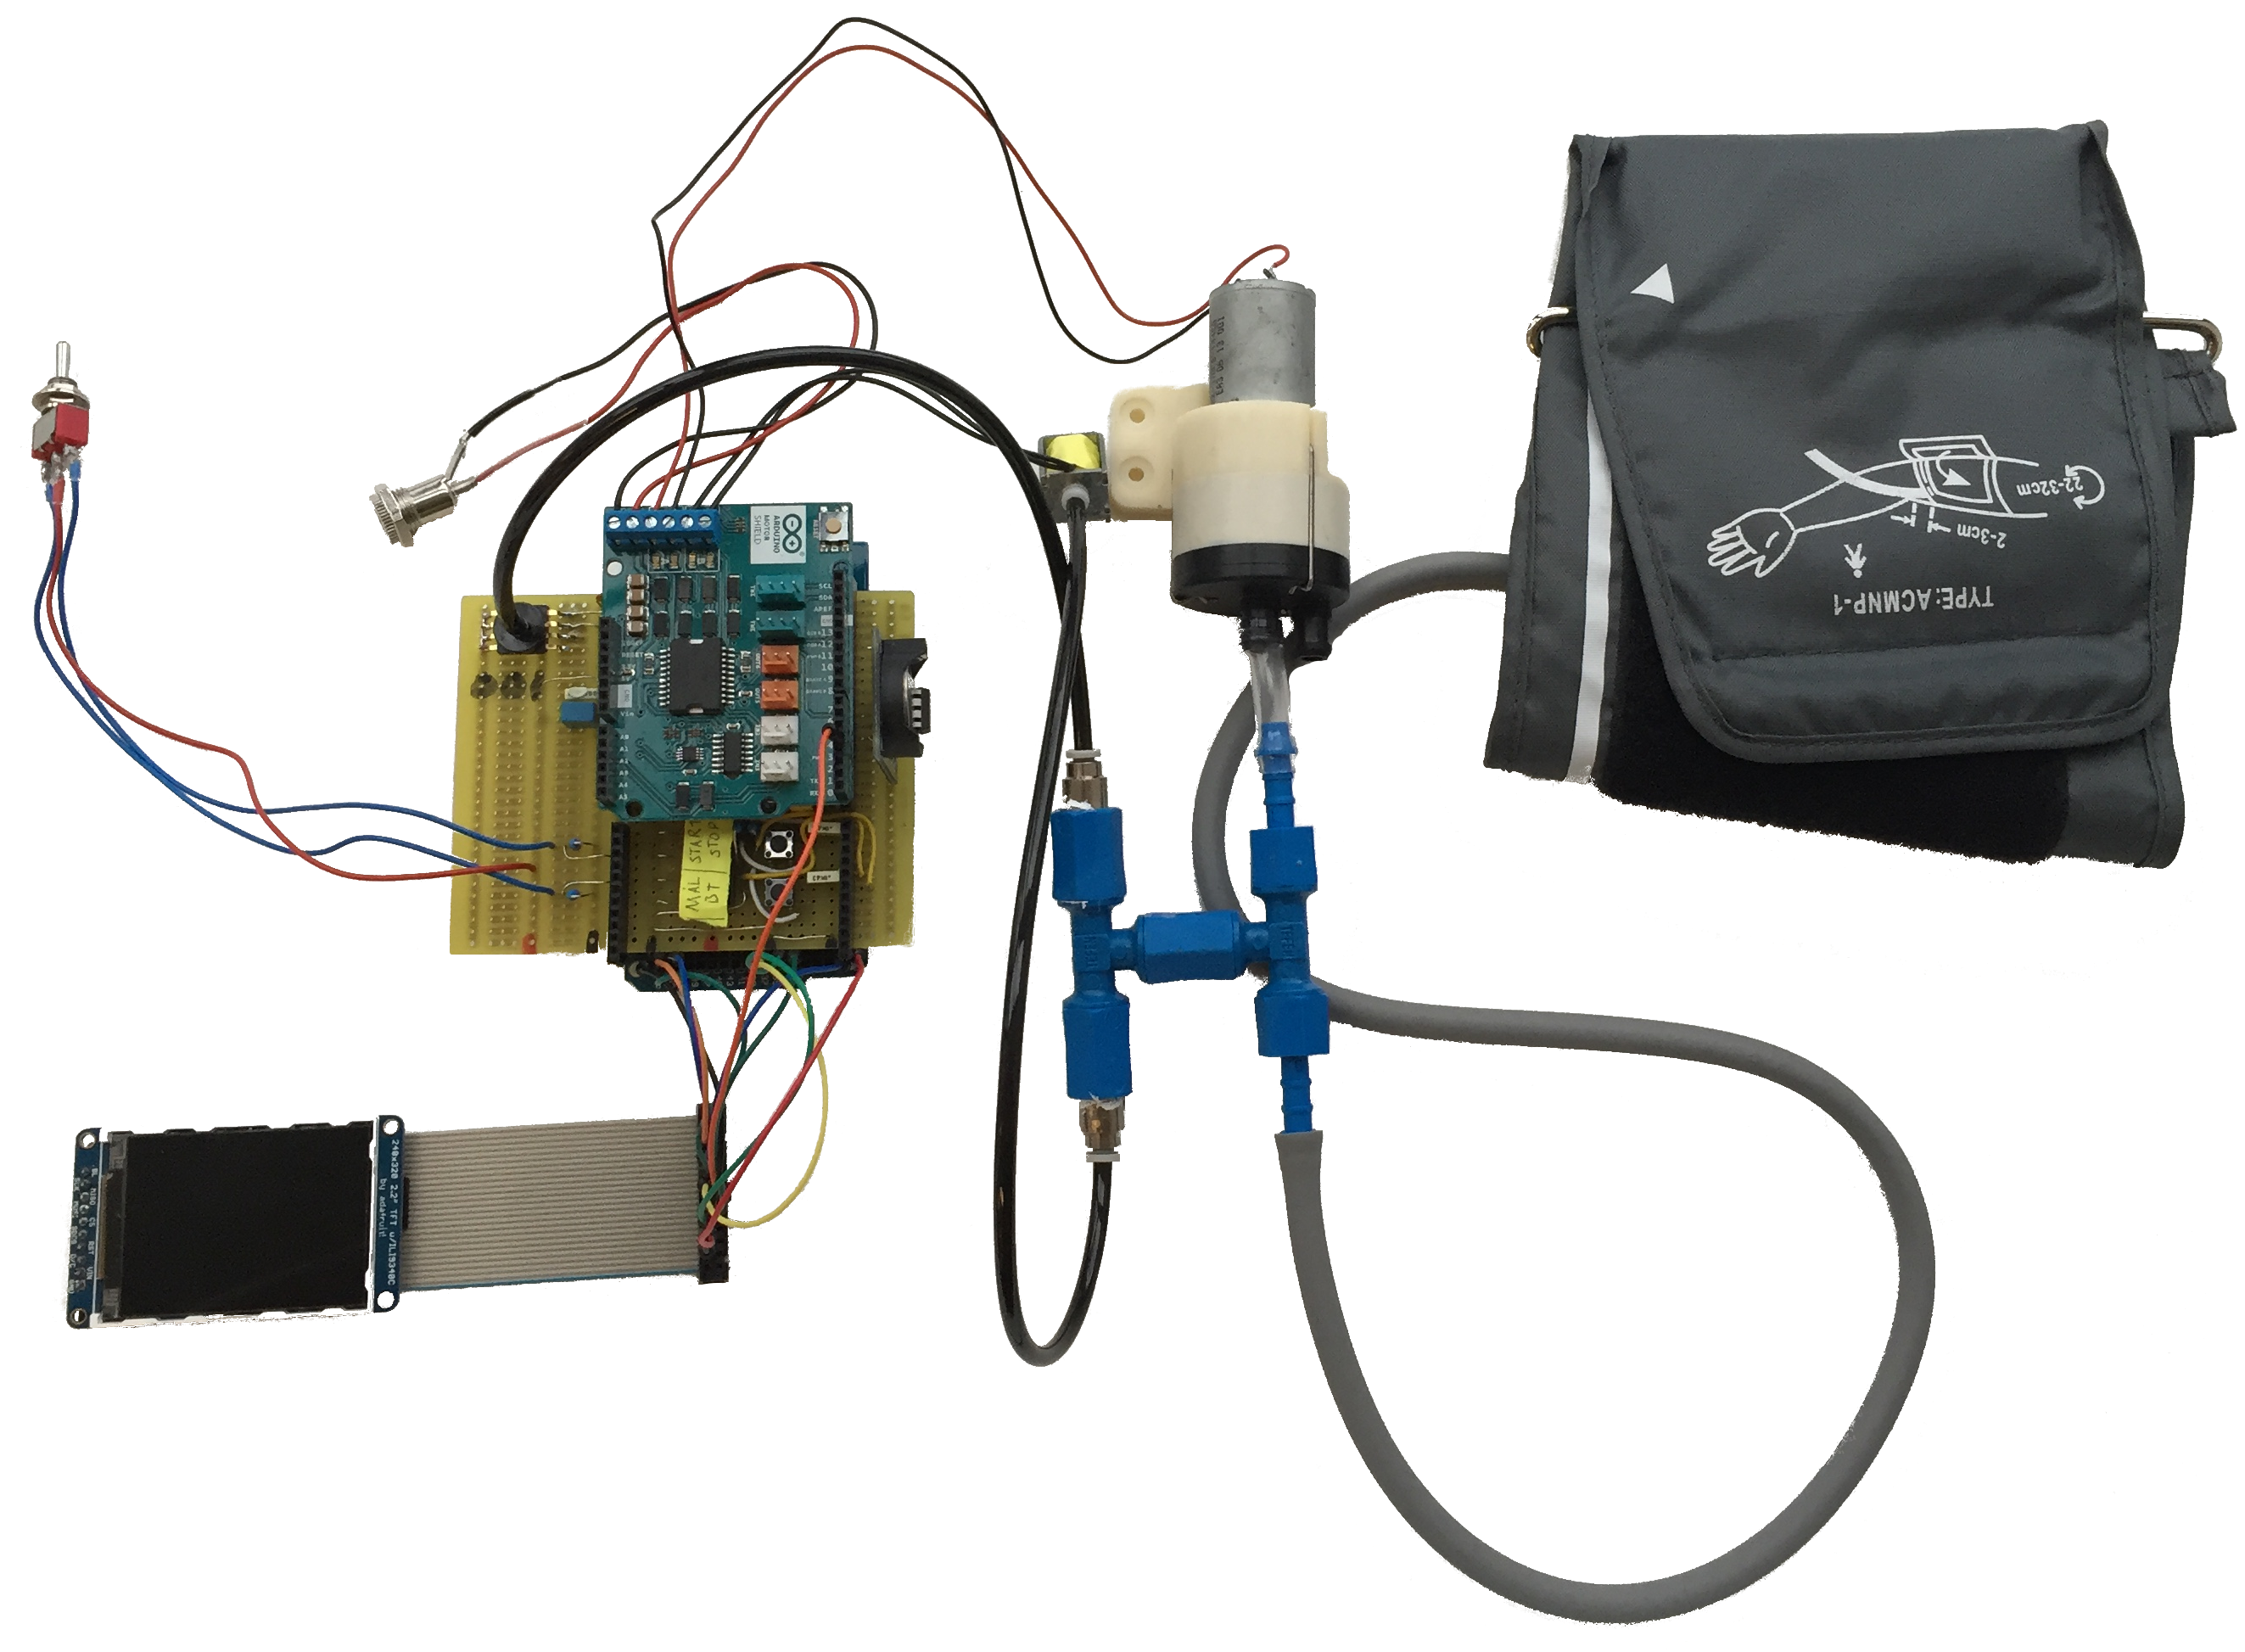
\includegraphics[width=0.9\textwidth]{formalia/forsidebillede.png}

\vspace{1cm} 
\textsc{\Large Bachelorprojekt \\
Gruppe 15155 \\
Karl-Johan Schmidt \\
Simon Vammen Grønbæk \\
Ingeniørhøjskolen, Aarhus Universitet \\
Efteråret 2015 \\}
\end{flushright}

	
	%Title page
	% Dette er et titelblad designet til videregående uddannelser på et universitet
% Filen kræver:
% Universitetets logo:  AU-logo-DK eller AU-logo-DK
% Synopsis: En fil ved navn synopsis.tex

% Udarbejdet af: Jesper Nørgaard (jesper@noergaard.eu) 10. april 2012

\phantomsection
\pdfbookmark[0]{Titelblad}{titelblad}
\thispagestyle{empty}

\begin{minipage}[t]{0.48\textwidth}
\vspace*{-8pt}			

\includegraphics[height=2.5cm]{filer/AU-logo-DK}
\end{minipage}
\hfill
\begin{minipage}[t]{0.48\textwidth}
{\small 
\textbf{Ingeniørhøjskolen Aarhus}\\
Finlandsgade 22 \\
8200 Aarhus N \\
Tlf: 8715 0000 \\
http://www.ase.au.dk/}
\end{minipage}

\vspace*{1cm}

\begin{minipage}[t]{0.48\textwidth}
\textbf{Titel:} \\[5pt]\bigskip\hspace{2ex}
System design

\textbf{Projekt:} \\[5pt]\bigskip\hspace{2ex}
Remote Ischemic Conditioning

\textbf{Projektperiode:} \\[5pt]\bigskip\hspace{2ex}
Juli 2015 - December 2015

\textbf{Projektgruppe:} \\[5pt]\bigskip\hspace{2ex}
15155

\textbf{Deltagere:} \\[5pt]\hspace*{2ex}
Simon Vammen Grønbæk\\\hspace*{2ex}
Karl-Johan Schmidt \\\hspace*{2ex}


\textbf{Vejledere:} \\[5pt]\hspace*{2ex}
Peter Johansen \\\bigskip\hspace{2ex}

\textbf{Projektudbyder:} \\[5pt]\hspace*{2ex}
Rolf Blauenfeldt\\\bigskip\hspace{2ex}
\vspace*{4cm}

\textbf{Versionsnummer: 0.5} \\
\textbf{Sidetal: \pageref{lastPage}} \\
\textbf{Afsluttet 16-12-2015}

\end{minipage}
\hfill
\begin{minipage}[t]{0.483\textwidth}
	\textbf{Godkendelse:}\vspace{1cm}
\begin{table}[H]
	\centering
	\begin{tabular}{c}
		\underline{\phantom{mmmmmmmmmmmmmm}}  \\
		Karl-Johan Schmidt \vspace{2cm}\\
		\underline{\phantom{mmmmmmmmmmmmmm}} \\
		Simon Vammen Grønbæk \vspace{2cm}	\\
		\underline{\phantom{mmmmmmmmmmmmmm}} \\
		Peter Johansen \vspace{2cm}	\\
		\underline{\phantom{mmmmmmmmmmmmmm}} \\
		Rolf Blauenfeldt \vspace{2cm}	\\
	\end{tabular}
\end{table}
\end{minipage}

\vfill


	
	\newpage
	\tableofcontents*{}
	\newpage
	
	%Indledning
	\chapter{Indledning}
Neurologisk afdeling på Aarhus Universitetshospital skal i et kommende studie, undersøge effekten af \textit{Remote Ischemic Pre- og Postcondtioning}. \textit{Remote ischemic conditiong (RIC)} er en behandlingsform, som har vist lovende resultater i forebyggelse og behandling af patienter med blodprop i hjertet. Studiet ønsker at undersøge om denne behandlingsform kan have samme gavnlige effekt på patienter med apopleksi. For at studiet skal kunne gennemføres, har afdelingen kontaktet Ingeniørhøjskolen, Aarhus Universitet, omkring udvikling af det apparat som skal udføre RIC behandlingen. Denne udviklingsopgave blev til dette bachelorprojekt. 

\section{Formål}
Formålet med denne projektrapport er at beskrive projektforløbet i forbindelse med udviklingen af \textit{Konditioneringsapparatet}. Rapport beskriver den faglige baggrund for projektet og behovet for et modificeret blodtryksapparat (konditioneringsapparat). Hernæst gennemgås hvilke afgrænsninger som projektgruppen har foretaget. Ydermere er formålet med rapporten, at sikre læseren har en forståelse for hvilke metoder der er anvendt i projektforløbet, samt resultatet og diskussion af den opnåede prototype. 

\section{Læsevejledning}
Projektrapporten skal læses som resultatet af projektforløbet. Rapporten er opdelt i følgende kapitlerne;

	\begin{longtable}{ p{0.14\textwidth} p{0.8\textwidth} } 
		Kapitel 1 & Præsentation af indelende punkter omkring bachelorprojektet \textit{Remote ischemic conditioning}\\
		Kapitel 2 & Her beskrivende den viden, der ligger til grund for forståelsen af projektet. \\
		Kapitel 3 & Beskrivelse af problemformuleringen, som er udarbejdet i samarbejde med kunden og vejleder\\
		Kapitel 4 & Præsentation af hvilke område, hvor projektet er blevet afgrænset\\
		Kapitel 5 & Giver en kort beskrivelse af den udviklede prototype\\
		Kapitel 6 & Redegørelse for hvilke ingeniørfaglige metoder projektet har gjort brug af \\
		Kapitel 7 & Præsentation af det central opnåede resultater ved produktudviklingen og projektforløbet\\
		Kapitel 8 & Beskrivelse og gennemgang af diskussion punkter omkring de central resultater\\
		Kapitel 9 & Redegøre for fremtiden for prototypen\\
		Kapitel 10& Indeholder en opsamling og konklusion på projektforløbet og prototypen\\
	\end{longtable}

\subsubsection{Appendiks}
Appendiks afsnittet indeholder logbog, tidsplan, samarbejdsaftale mm. Dette afsnit skal læses som dokumentation for projektforløbet

\subsubsection{Udviklingsdokumentation}
Foruden dokumentationsrapporten består projektgruppens skriftlige produkt også af en udviklingsdokumentation. Dette er et dokument, som giver læseren fuld indblik i udviklingsfasen af \textit{Konditioneringsapparatet}. Dokument består af 4 underdokumenter, hhv. kravspecifikation, accepttest, system design og implementering. 

Dokumentationsrapporten bygger på udviklingsdokumentationen, som af denne grund er fungerende som opslagsdokument for dokumentationsrapporten. 




	
	\chapter{Systemets dele} \label{title:systemPart}
Dette afsnit beskriver systemet, \textit{Konditioneringsapparats}, fysiske dele og deres funktionalitet.

\section{Microcontroller}
Styring af alle systemets dele. Her processeres brugerens interagering med \textit{Kondtioneringsapparat} og handlingerne eksekveres. Microcontrolleren er en AtMega32 og styringen af chippen skrives i C++.

\section{Manchetten}
Trykmanchet til at skabe okklusion af armen. Manchetten skal kunne holde trykket, som skabes af pumpen. Manchetten kobles til apparatet via en lufttæt slange. 

\section{User interface, knapper og displays}
Brugerfladen består af et display hvor blodtryk, antal okklusioner, resterende tid og mm. vises. Displayet skal bruges til at give brugeren feedback og fx. informere det medicinske personale hvor lang tid der er indtil konditioneringen er færdig. 

På \textit{Konditioneringsapparatet} er der to knapper [Start/Stop] og [Mål blodtryk]. Disse knapper bruges til at initierer konditioneringsbehandling, blodtryksmålinger og okklusionstræning. På bagsiden af apparatet sidder desuden en Modeswitch, hvor brugeren kan skifte mellem \textit{Okklusionstræning}, \textit{Konditionering}, eller \textit{Setup}. 

\section{Power system}
Forsyning af systemet foregår med 8 batterier af typen AAA for at opnå en spænding på 12V. Systemet forsynes med en batteriløsning, for at gøre det mere mobilt.  

Foruden at forsyne apparatet, er power system også bestående af et motorshield. Når microcontroller fx ønsker at starte pumpen, sørger motorshieldet for at levere det korrekte spænding. 

\section{Pumpe}
Består af en motor og et luftindtag. Pumpe kan både bruges til at skabe tryk og vakuum. Pumpen skal bruges til at inflatere manchetten til måling af blodtryk og til okklusion af armen, både under konditionering og under træning. Pumpen skal forsynes med 12 V og hastigheden kan styres med PWM. 

\section{Ventil}
Ventilen indgår i systemet til at nedregulere trykket i manchetten. Ventilen er “Normally closed”. Funktionen af ventilen under en blodtryksmåling er gradvis at lukke trykket ud, så det er muligt at registrere oscillationerne og det aktuelle tryk. Under okklusion har ventilen en anden funktion, her indgår ventilen i reguleringen.

\section{Tryksensor}
En 5 V tryksensor, der bruges til registrering af trykket i manchetten og til efter regulering. Tryksensoren skal også registrere oscillationerne, der skabes i manchetten når trykket er omkring systolisk niveau og ved middeltrykket. Ved okklusionstræning skal tryksensoren bruges til at holde trykket konstant omkring 100 mmHg.

\section{SD kort}
Apparatet udstyres med ekstern hukommelse, for at det er muligt for \textit{Konditioneringsapparatet} at gemme information omkring behandlingsforløbet. Der er valgt et SD kort, fordi når behandlingen er færdig, er det muligt at skifte SD kortet ud, og på den måde have backup af information og det er nemmere at overføre informationen. 

\section{Pulsoximeter}
Som undersystemet i \textit{Konditioneringsapparatet} indgår et pulsoximeter, der skal bruges til overvågning af patientens tilstand under konditioningsbehandling. Pulsoximeteret leverer en saturation efter hver endt okklusion og den saturation er med til at bestemme om patientens kredsløb kan tåle behandlingen.
	
	\chapter{Arkitektur}

\section{4+1 view architecture} \label{title:viewArc}
Denne model beskriver arkitekturen af software baserede systemer. For at skabe en fyldestgørende gennemgang af systemet gøres brug af fire forskellige synsvinkler. Disse synsvinkler har til formål at  tilfredsstille alle interessenter og sørge for at alle parter forstår systemet. Eksempler på parter kunne være kunden, projektleder eller udviklere. Med udgangspunkt i use cases består modellen af følgende punkter: 

\begin{figure}[H]
	\includegraphics[width=\textwidth]{SystemArkitektur/filer/4plus1model.png}
	\caption{4+1 view architecture model. Kilde: \cite{RefWorks:10}}\label{fig:4plus1model}
\end{figure}

\textit{Logical view:} Denne synsvinkel beskriver systemets funktionalitet via centrale elementer, mekanismer og stadier.

\textit{Process view:} Beskæftiger sig med de dynamiske aspekter af systemet, forklarer system processer, hvordan de kommunikerer, og fokuserer på systemets opførsel i drift.

\textit{Implementation view:} Denne vinkel involverer udviklerens perspektiv og beskæftiger sig med hvordan software implementeres.

\textit{Deployment view:} Beskriver systemet fra en fysisk synsvinkel, blandt andet hvordan eksekveringen af softwares skal foregå på apparatet og hvordan systemets fysisk setup skal ser ud. 

Modellen “\textit{4+1 view architecture}” er beregnet primært til software baserede udviklingsprojekter og derfor bruges den som en retningslinje og inspiration til systemet arkitekturen. Da Konditioneringsapparatet er en prototype som involvere både hardware og software er modellen blevet tilpasset dertil. Endvidere vil systemet blive præsenteret og gennemgået ved hjælp af SysML standarden, selvom modellen er lavet til UML.



\section{Logic}

\subsection{Block definition diagram}
Blokdiagrammer giver et indblik på den overordnede strukturen af \textit{Konditioneringsapparatet}.  Hver kasse skal ses som en del der indgår i systemet

\subsection{Domænemodel}
Diagrammer beskriver det systemet som helhed. Ved gennemgang af alle use cases findes væsentlig navneord og disse oprettet som konceptuelle klasser. Det konceptuelle klasser er derefter oversat til engelsk

\subsection{State machine diagram}

\subsubsection{Boot}
\includegraphics[width=\textwidth]{pdfs/STM_BOOT-crop.pdf} 

\subsubsection{Konditionering}
Ved knap tryk på [Start/Stop] \\
\includegraphics[width=\textwidth]{pdfs/STM_Konditionering1-crop.pdf}

Ved knap tryk på [Mål blodtryk] \\
\includegraphics[width=\textwidth]{pdfs/STM_Konditionering2-crop.pdf}

\subsubsection{Okklusion}
\begin{center}
\includegraphics[width=0.5\textwidth]{pdfs/STM_Okklusion-crop.pdf}
\end{center}

\subsubsection{Setup}
\includegraphics[width=\textwidth]{pdfs/STM_Setup-crop.pdf}


\section{Process}

\subsection{Sekvensdiagrammer}
Der er udarbejdet et sekvensdiagram for hver use case. Et sekvensdiagram viser hvordan systemets dele og aktører interagerer med hinanden, og hvilke processer der sker ved disse interaction. Det er beskrevet som sekventiel process og der illustreret diagrammet også hvilke rækkefølge processerne skal eksekveres i. 
Fordi at simplificeret store sekvensdiagrammer gør nogle af dem brug af andre use case, dette ses fx. i sekvensdiagrammet for use case 1. 

\subsection{Konditionering - UC1}
\includegraphics[width=\textwidth]{pdfs/SD_UC1-crop.pdf}

\subsection{Initialiser blodtryksmåling - UC2}
\includegraphics[width=\textwidth]{pdfs/SD_UC2-crop.pdf}

\subsection{Mål blodtryk - UC3}
\includegraphics[width=\textwidth]{pdfs/SD_UC3-crop.pdf}

\subsection{Overfør data - UC4}
\includegraphics[width=\textwidth]{pdfs/SD_UC4-crop.pdf}

\subsection{Sikkerhedskontrol med pulsoximeter - UC5}
Mangler stadig...

\subsection{Okklusionstræning - UC6}
\includegraphics[width=\textwidth]{pdfs/SD_UC6-crop.pdf}

\subsection{Afbryd - UC7}
\includegraphics[width=\textwidth]{pdfs/SD_UC7-crop.pdf}

\subsection{Setup - UC8}
\includegraphics[width=\textwidth]{pdfs/SD_UC8-crop.pdf}


\section{Implementation}

\subsection{Hardware}
Diagrammet viser interaktioner mellem systemets hardware dele \\
\includegraphics[width=\textwidth]{pdfs/InternalBlockdiagram(Hardware).png}
(Skal rettes til PDF)

\subsubsection{Beskrivelse af hardware}
INDSÆT reference til kapitel 2

\subsubsection{Arduino Mega og Motor Shield}
\includegraphics[width=\textwidth]{pdfs/MegaPlusShield-crop.pdf}

\subsection{Software}

\section{Deployment}
Da produktet Konditioneringsapparat er en prototype beskæftiger projektet sig ikke med de redskaber der bruges i deployment view. Dette view beskriver blandt andet hvordan software mappes på hardware, kaldet et deployment diagram. Konditioneringsapparatet består kun af én software eksekverende enhed og derfor er dette overflødigt at beskrive. 


\end{document}
\stopcontents[sd]
\resumecontents[overall]
\newpage

\part{ Implementeringsdokument} \label{part:id}
\stopcontents[overall]
\startcontents[id]

 %	\thispagestyle{empty}
\begin{flushright}
\vspace{3cm}

\phantom{hul}

\phantom{hul}

\phantom{hul}

\textsl{\Huge Remote Ischemic Conditioning} \\ \vspace{1cm}
\textsl{\Huge Udviklingsdokumentation} \\ \vspace{1cm}

\rule{\textwidth}{3mm} \\ \vspace{1.5cm}
\vspace{1cm}

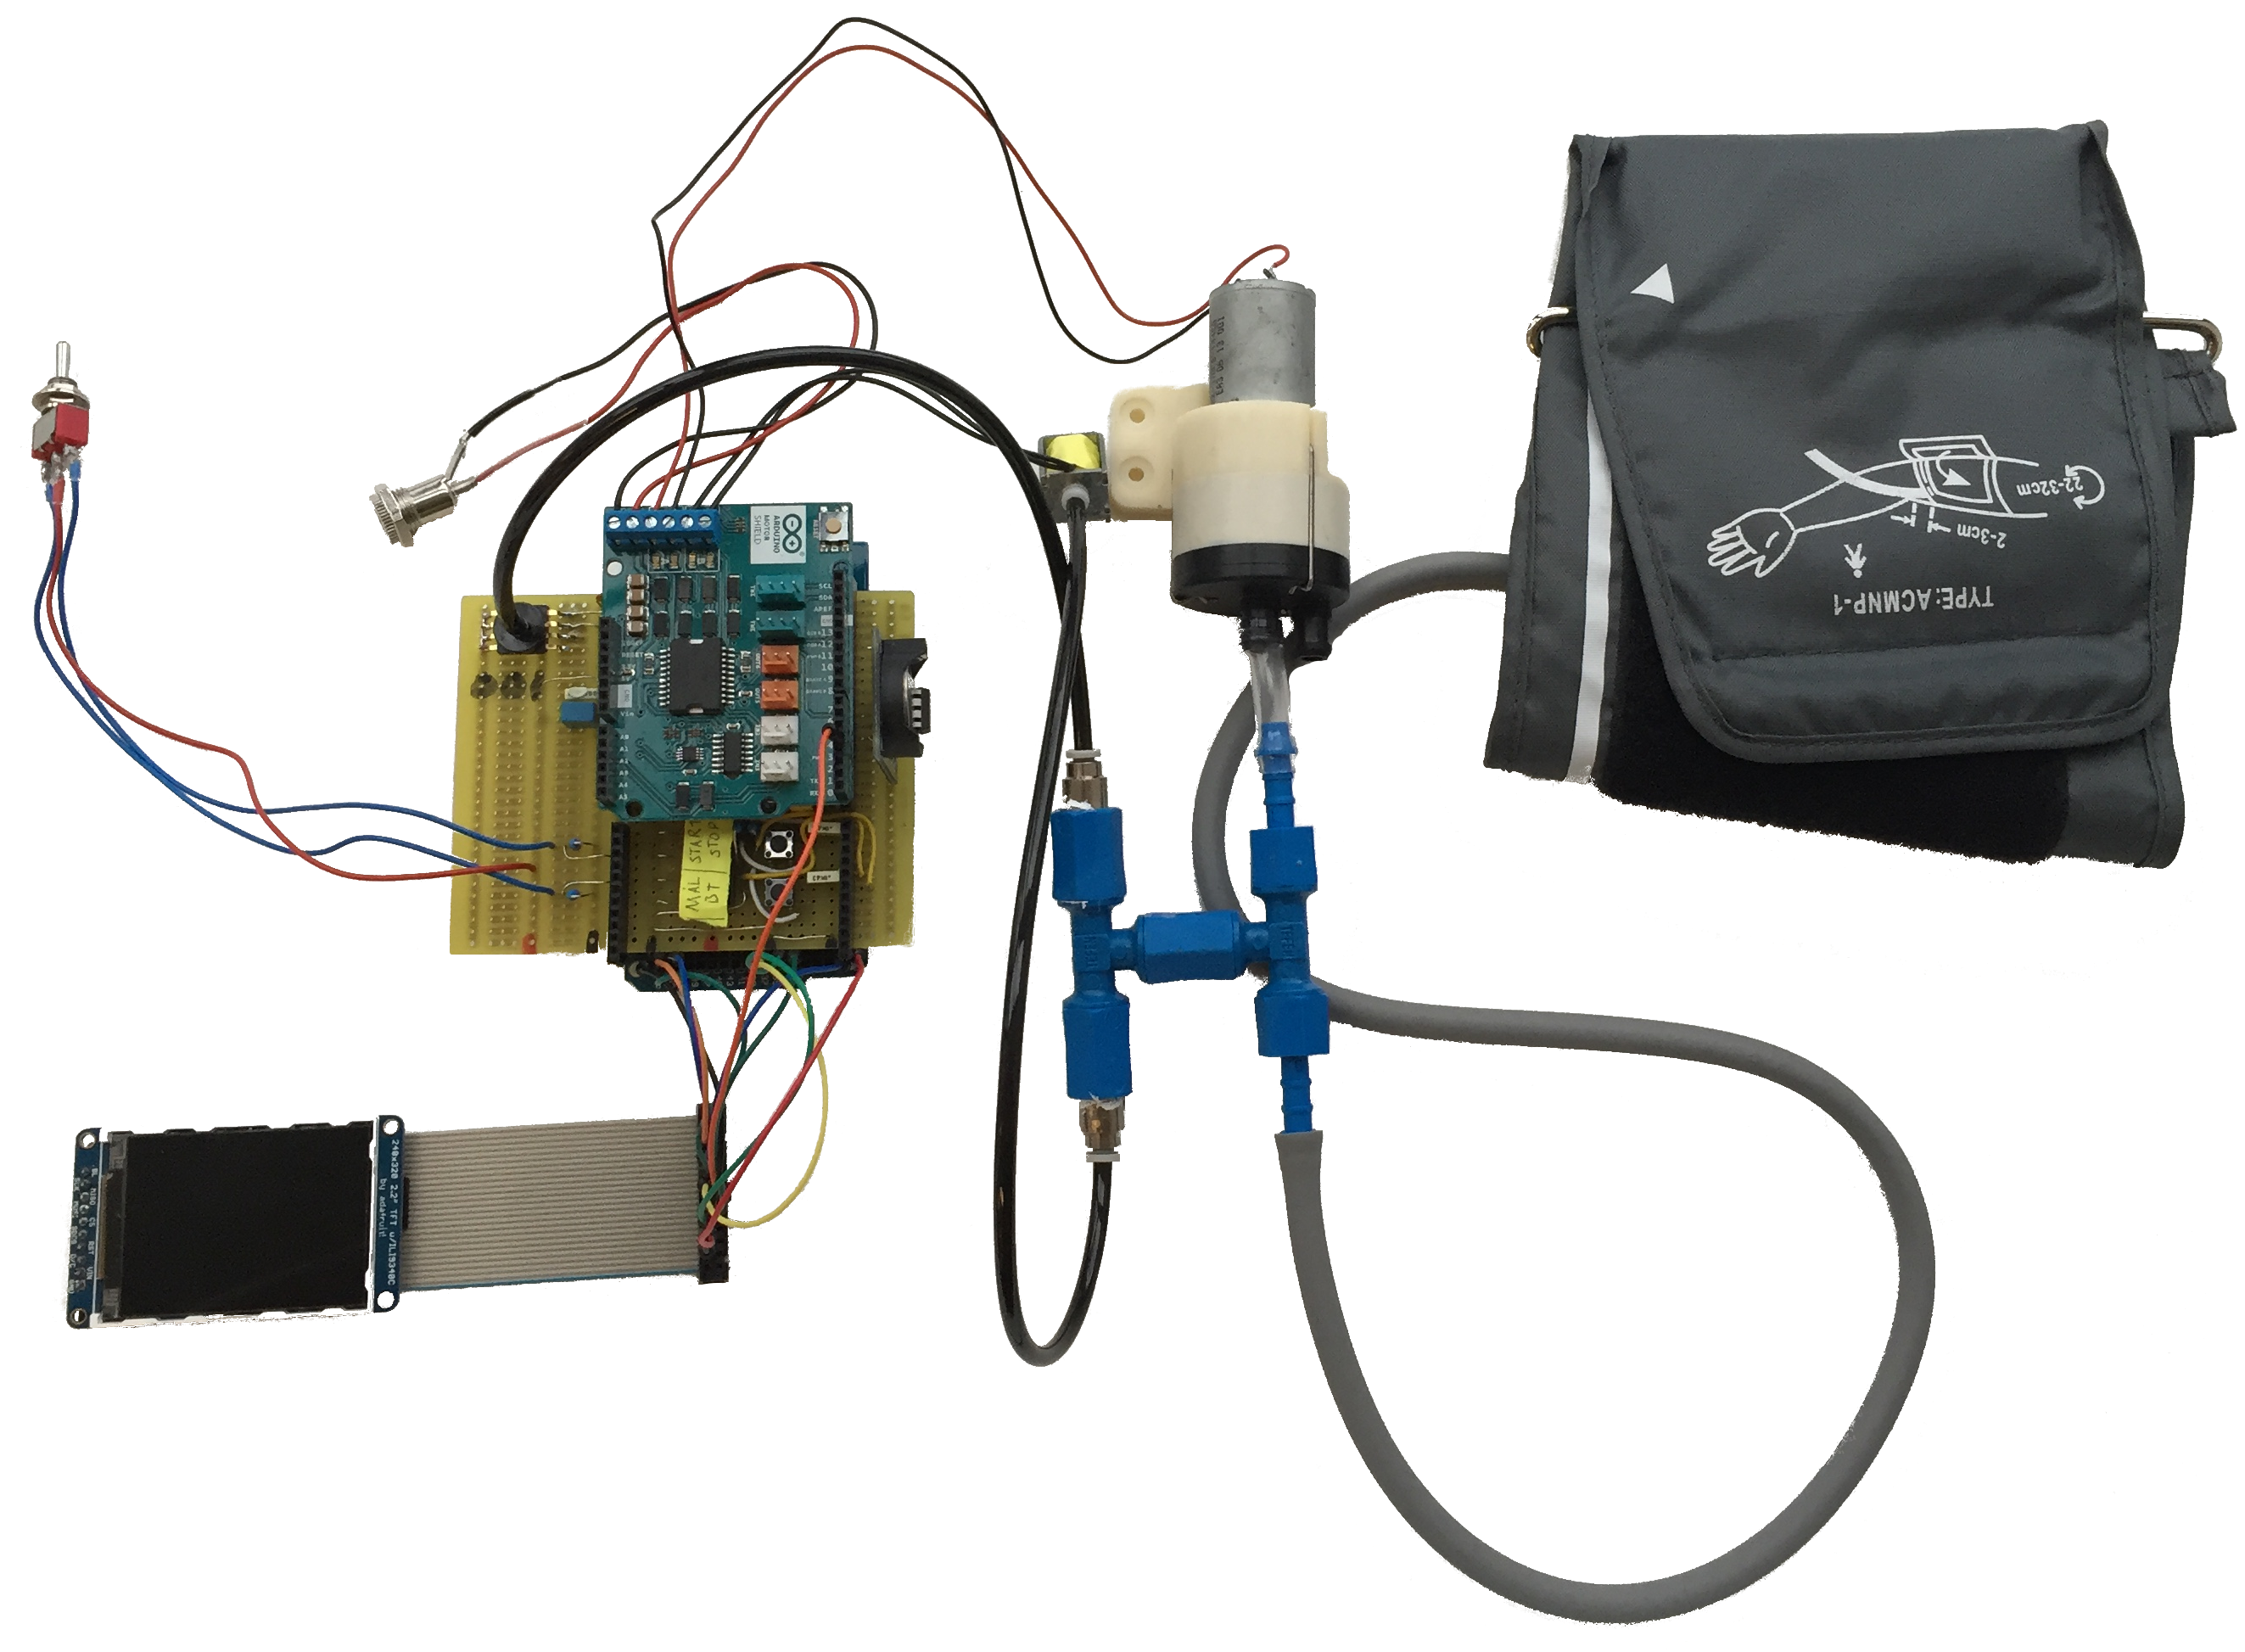
\includegraphics[width=0.9\textwidth]{formalia/forsidebillede.png}

\vspace{1cm} 
\textsc{\Large Bachelorprojekt \\
Gruppe 15155 \\
Karl-Johan Schmidt \\
Simon Vammen Grønbæk \\
Ingeniørhøjskolen, Aarhus Universitet \\
Efteråret 2015 \\}
\end{flushright}

%	% Dette er et titelblad designet til videregående uddannelser på et universitet
% Filen kræver:
% Universitetets logo:  AU-logo-DK eller AU-logo-DK
% Synopsis: En fil ved navn synopsis.tex

% Udarbejdet af: Jesper Nørgaard (jesper@noergaard.eu) 10. april 2012

\phantomsection
\pdfbookmark[0]{Titelblad}{titelblad}
\thispagestyle{empty}

\begin{minipage}[t]{0.48\textwidth}
\vspace*{-8pt}			

\includegraphics[height=2.5cm]{filer/AU-logo-DK}
\end{minipage}
\hfill
\begin{minipage}[t]{0.48\textwidth}
{\small 
\textbf{Ingeniørhøjskolen Aarhus}\\
Finlandsgade 22 \\
8200 Aarhus N \\
Tlf: 8715 0000 \\
http://www.ase.au.dk/}
\end{minipage}

\vspace*{1cm}

\begin{minipage}[t]{0.48\textwidth}
\textbf{Titel:} \\[5pt]\bigskip\hspace{2ex}
System design

\textbf{Projekt:} \\[5pt]\bigskip\hspace{2ex}
Remote Ischemic Conditioning

\textbf{Projektperiode:} \\[5pt]\bigskip\hspace{2ex}
Juli 2015 - December 2015

\textbf{Projektgruppe:} \\[5pt]\bigskip\hspace{2ex}
15155

\textbf{Deltagere:} \\[5pt]\hspace*{2ex}
Simon Vammen Grønbæk\\\hspace*{2ex}
Karl-Johan Schmidt \\\hspace*{2ex}


\textbf{Vejledere:} \\[5pt]\hspace*{2ex}
Peter Johansen \\\bigskip\hspace{2ex}

\textbf{Projektudbyder:} \\[5pt]\hspace*{2ex}
Rolf Blauenfeldt\\\bigskip\hspace{2ex}
\vspace*{4cm}

\textbf{Versionsnummer: 0.5} \\
\textbf{Sidetal: \pageref{lastPage}} \\
\textbf{Afsluttet 16-12-2015}

\end{minipage}
\hfill
\begin{minipage}[t]{0.483\textwidth}
	\textbf{Godkendelse:}\vspace{1cm}
\begin{table}[H]
	\centering
	\begin{tabular}{c}
		\underline{\phantom{mmmmmmmmmmmmmm}}  \\
		Karl-Johan Schmidt \vspace{2cm}\\
		\underline{\phantom{mmmmmmmmmmmmmm}} \\
		Simon Vammen Grønbæk \vspace{2cm}	\\
		\underline{\phantom{mmmmmmmmmmmmmm}} \\
		Peter Johansen \vspace{2cm}	\\
		\underline{\phantom{mmmmmmmmmmmmmm}} \\
		Rolf Blauenfeldt \vspace{2cm}	\\
	\end{tabular}
\end{table}
\end{minipage}

\vfill


\newpage
\printcontents[id]{ }{0}{\chapter*{Indholdsfortegnelse}}
\newpage
	
	\chapter{Indledning}
Neurologisk afdeling på Aarhus Universitetshospital skal i et kommende studie, undersøge effekten af \textit{Remote Ischemic Pre- og Postcondtioning}. \textit{Remote ischemic conditiong (RIC)} er en behandlingsform, som har vist lovende resultater i forebyggelse og behandling af patienter med blodprop i hjertet. Studiet ønsker at undersøge om denne behandlingsform kan have samme gavnlige effekt på patienter med apopleksi. For at studiet skal kunne gennemføres, har afdelingen kontaktet Ingeniørhøjskolen, Aarhus Universitet, omkring udvikling af det apparat som skal udføre RIC behandlingen. Denne udviklingsopgave blev til dette bachelorprojekt. 

\section{Formål}
Formålet med denne projektrapport er at beskrive projektforløbet i forbindelse med udviklingen af \textit{Konditioneringsapparatet}. Rapport beskriver den faglige baggrund for projektet og behovet for et modificeret blodtryksapparat (konditioneringsapparat). Hernæst gennemgås hvilke afgrænsninger som projektgruppen har foretaget. Ydermere er formålet med rapporten, at sikre læseren har en forståelse for hvilke metoder der er anvendt i projektforløbet, samt resultatet og diskussion af den opnåede prototype. 

\section{Læsevejledning}
Projektrapporten skal læses som resultatet af projektforløbet. Rapporten er opdelt i følgende kapitlerne;

	\begin{longtable}{ p{0.14\textwidth} p{0.8\textwidth} } 
		Kapitel 1 & Præsentation af indelende punkter omkring bachelorprojektet \textit{Remote ischemic conditioning}\\
		Kapitel 2 & Her beskrivende den viden, der ligger til grund for forståelsen af projektet. \\
		Kapitel 3 & Beskrivelse af problemformuleringen, som er udarbejdet i samarbejde med kunden og vejleder\\
		Kapitel 4 & Præsentation af hvilke område, hvor projektet er blevet afgrænset\\
		Kapitel 5 & Giver en kort beskrivelse af den udviklede prototype\\
		Kapitel 6 & Redegørelse for hvilke ingeniørfaglige metoder projektet har gjort brug af \\
		Kapitel 7 & Præsentation af det central opnåede resultater ved produktudviklingen og projektforløbet\\
		Kapitel 8 & Beskrivelse og gennemgang af diskussion punkter omkring de central resultater\\
		Kapitel 9 & Redegøre for fremtiden for prototypen\\
		Kapitel 10& Indeholder en opsamling og konklusion på projektforløbet og prototypen\\
	\end{longtable}

\subsubsection{Appendiks}
Appendiks afsnittet indeholder logbog, tidsplan, samarbejdsaftale mm. Dette afsnit skal læses som dokumentation for projektforløbet

\subsubsection{Udviklingsdokumentation}
Foruden dokumentationsrapporten består projektgruppens skriftlige produkt også af en udviklingsdokumentation. Dette er et dokument, som giver læseren fuld indblik i udviklingsfasen af \textit{Konditioneringsapparatet}. Dokument består af 4 underdokumenter, hhv. kravspecifikation, accepttest, system design og implementering. 

Dokumentationsrapporten bygger på udviklingsdokumentationen, som af denne grund er fungerende som opslagsdokument for dokumentationsrapporten. 




	
	\chapter{Software}

\section{Klasse diagram}
Oversigtsklassediagram, se figur \ref{fig:classDiagramSimple}, som fortæller strukturen af namespaces og klasse, men for overskueligheden er alle metoder undladt, se disse under deres respektive afsnit
\begin{figure}[H]
	\includegraphics[width=\textwidth]{Implementeringsdokument/klassediagram_forsimplet-crop.pdf}
	\caption{Forsimplet klasse diagram}\label{fig:classDiagramSimple}
\end{figure}
\newpage

\section{Namespace: GUI Laget}

\begin{figure}[H]
	\includegraphics[width=\textwidth]{klassediagram_GUI-crop.pdf}
	\caption{Klasse diagram over namespacet GUI}\label{fig:classDiagramGUI}
\end{figure}

\subsection{Klasse: Display}
Denne klasse gør brug af to biblioteker for at kunne bruge TFT skærmen, henholdvis Adafruit\_GFX og Adafruit\_ILI9340. For at kunne kommunikere med displayet gøres der brug af disse bibliotekters indbyggede funktioner. Derfor oprettes et objekt af klassen Adafruit\_ILI9340 kaldet TFTscreen.

\subsubsection{Metode: initDisplay()}
\textbf{Parameter: } 
\\ \textbf{Returtype: } \textit{void}
\\ \textbf{Beskrivelse: } Her initieres skærmen med funktion \textit{.begin().} Rotationen og baggrundsfarven af skærmen sættes også når denne metode kaldes. Skærmrotationen er sat 3, hvilket betyder at skærmen er i “landscape mode”. 

\subsubsection{Metode: clearAreaDisp()}
\textbf{Parameter: } \textit{unsigned short pointX, unsigned short pointY, unsigned short width, unsigned short height}
\\ \textbf{Returtype: } \textit{void}
\\ \textbf{Beskrivelse: } Da skærmen baggrundsfarven er sat til sort, medtager denne metode 4 parameter hhv. start x-koordinat, start y-koordinat, bredde og højde. Disse parameter fortæller hvor en del af skærmen der skal farves sort, og dermed slette det område.

\subsubsection{Metode: initConditioning()}
\textbf{Parameter: }
\\ \textbf{Returtype: } \textit{void}
\\ \textbf{Beskrivelse: } Når denne metode kaldes skrives de “faste” værdier på skærmen til et konditioneringsforløb. På billedet nedenfor ses hvordan skærmen ser ud, når metoden er kørt. Et eksempel på hvordan der skrives tekst på skærmen: 
\begin{lstlisting}
TFTscreen.setTextColor(ILI9340_WHITE);  TFTscreen.setTextSize(2);
TFTscreen.setCursor(0, 0);
TFTscreen.println("ID: ");
\end{lstlisting}
Først fortælles hvilken farve teksten skal have, dernæst tekststørrelse og placering. Til sidst angives hvilken tekst der skal printes på skærmen

\begin{figure}[H]
	\includegraphics[width=\textwidth]{billeder/conditioning.png}
	\caption{Layout på displayet når initConditioning() bliver kaldt}\label{pic:conditiong}
\end{figure}

\subsubsection{Metode: initOcclusion()}
\textbf{Parameter: }
\\ \textbf{Returtype: } \textit{void}
\\ \textbf{Beskrivelse: }  Denne metode bruges til at opsætte skærmen for okklusionstræningsforløb. Der skrives tid og enheden for tryk på skærmen. Se billedet nedenfor for layoutet. 

\begin{figure}[H]
	\includegraphics[width=\textwidth]{billeder/occlusion.png}
	\caption{Layout på displayet når initOcclusion() bliver kaldt}\label{pic:occlusion}
\end{figure}

\subsubsection{Metode: initSetup()}
\textbf{Parameter: } 
\\ \textbf{Returtype: } \textit{void}
\\ \textbf{Beskrivelse: } Her opsættes skærmen for setup programmet. Teksten “\textit{Tid pr cyklus}” og “\textit{Antal cyklusser}” er faste værdi på skærmen. Men værdierne hentes fra logik laget, så de er opdateret. 

\begin{figure}[H]
	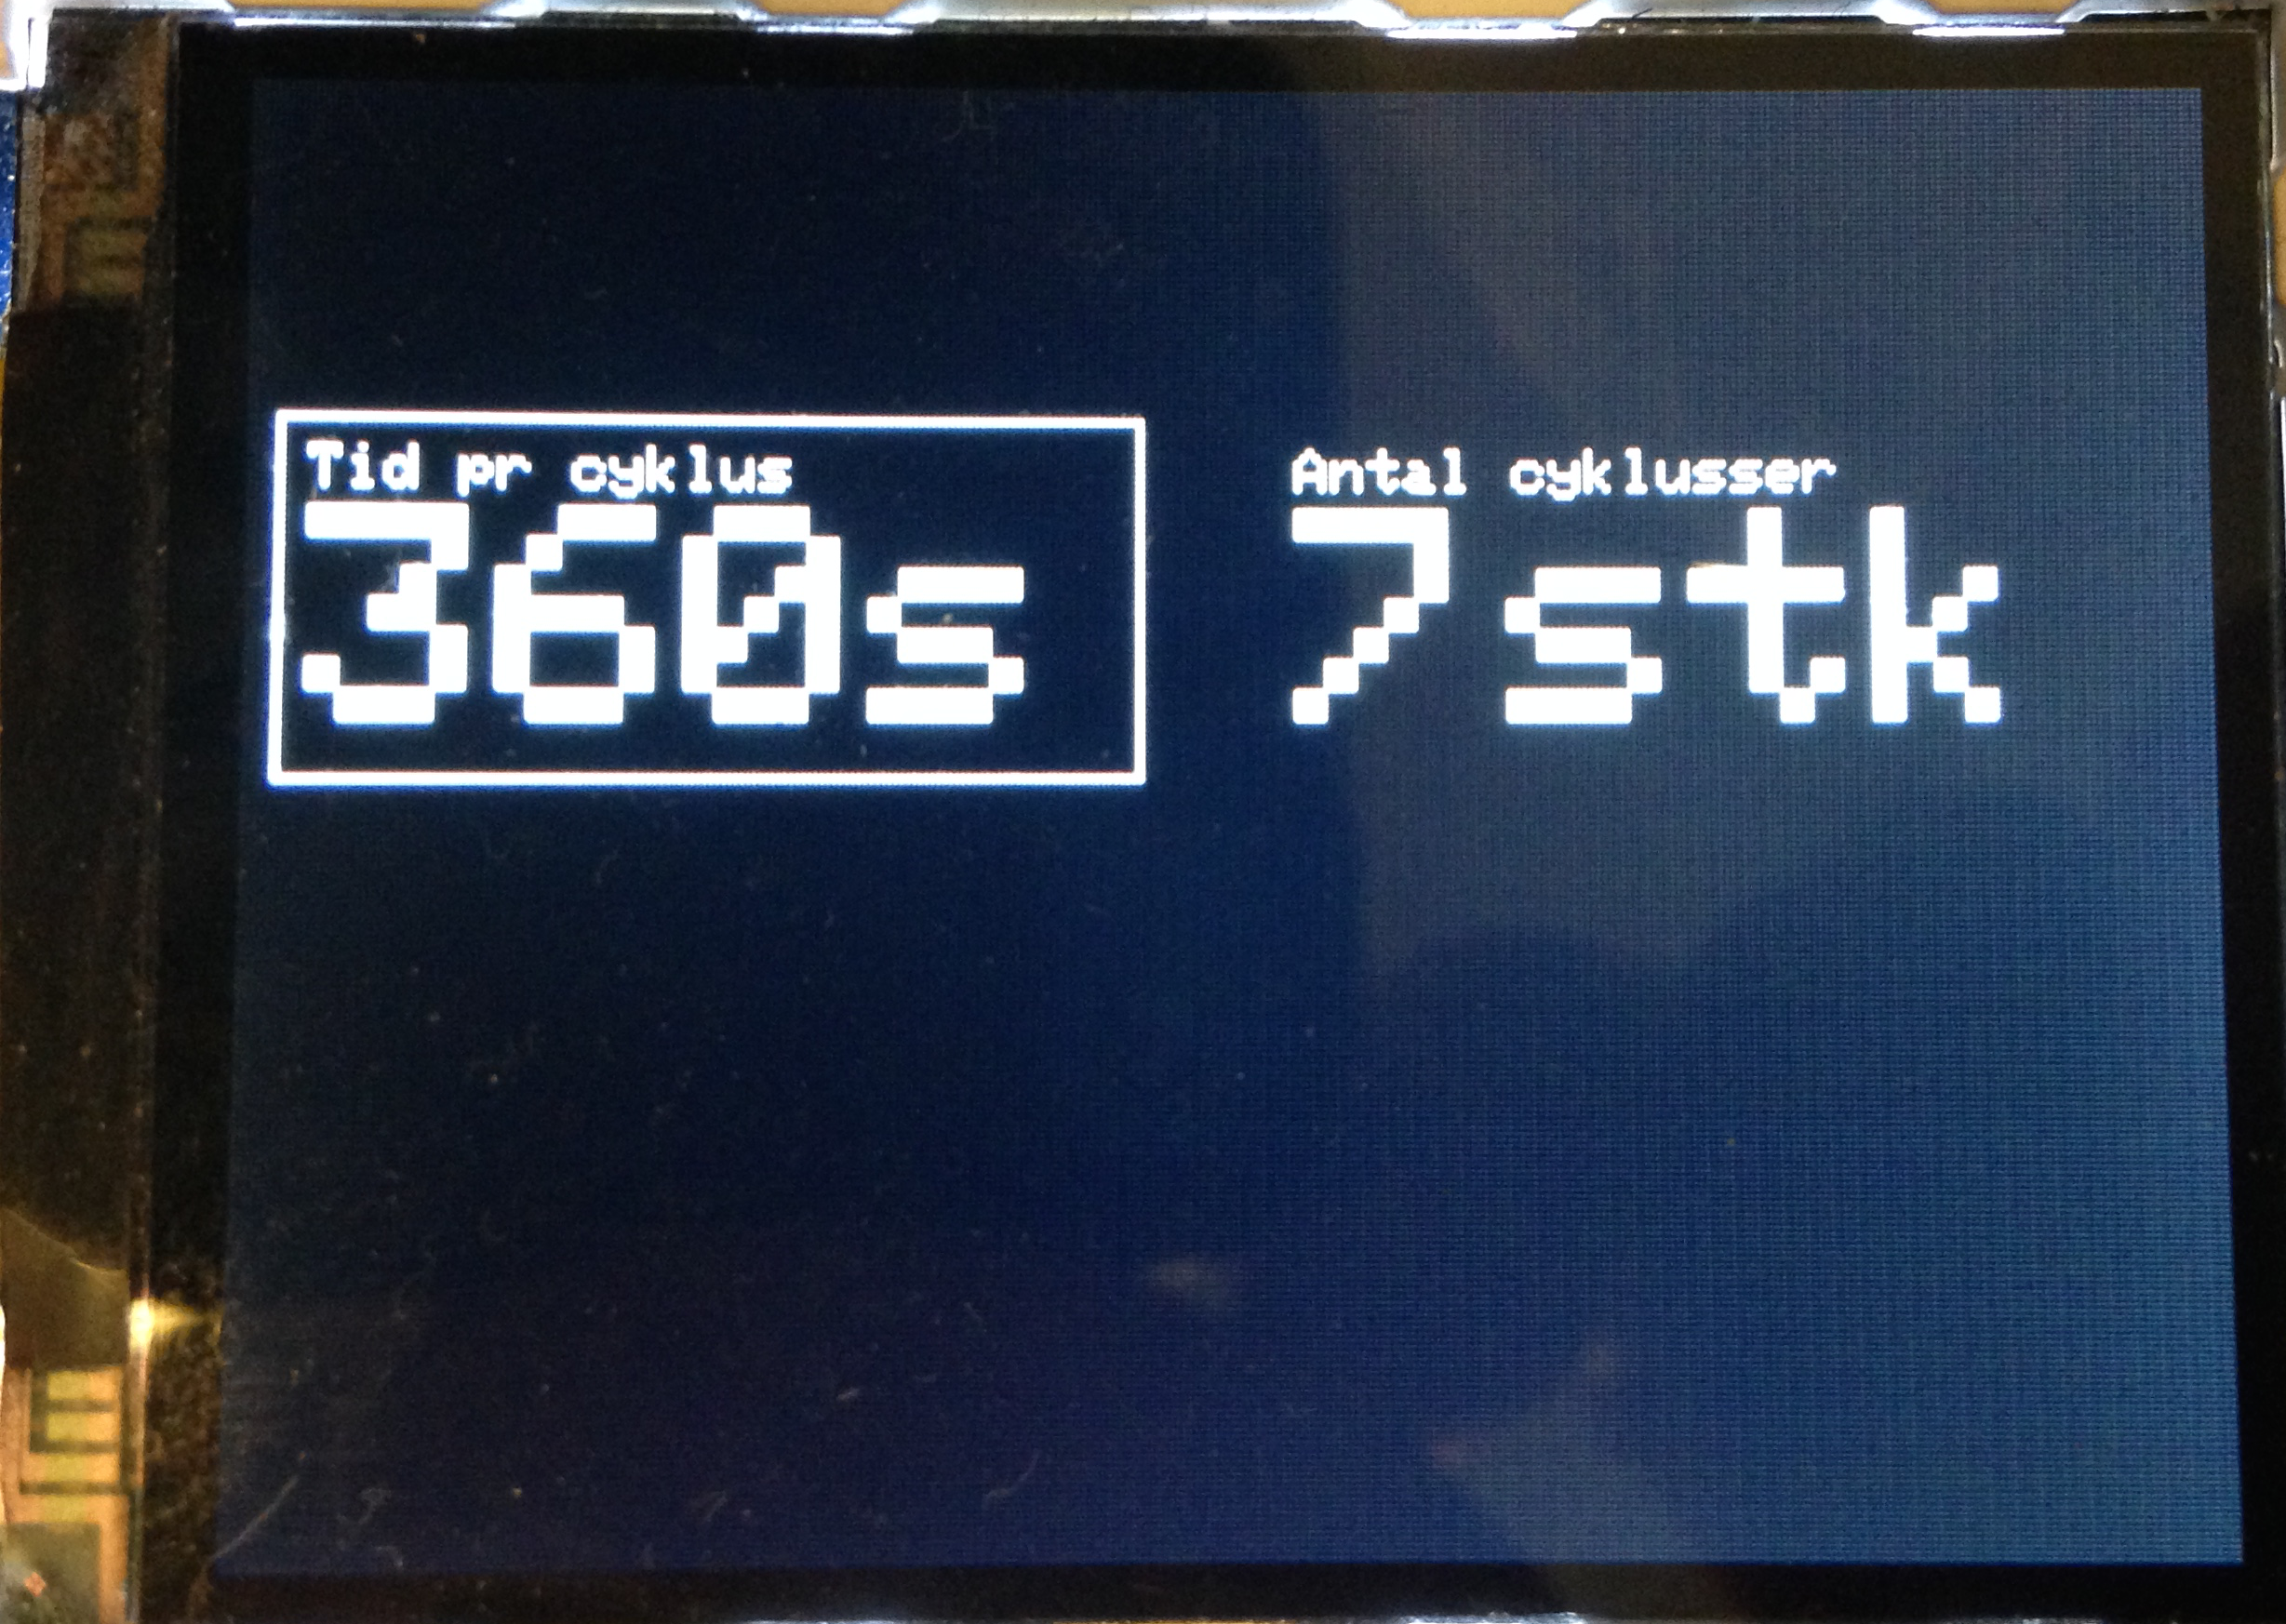
\includegraphics[width=\textwidth]{billeder/setup.png}
	\caption{Layout på displayet når initSetup() bliver kaldt}\label{pic:setup}
\end{figure}

\subsubsection{Metode: moveSquare()}
\textbf{Parameter: } \textit{unsigned short startX, unsigned short startY, unsigned short endX, unsigned short endY, unsigned short width, unsigned short height}
\\ \textbf{Returtype: } \textit{void}
\\ \textbf{Beskrivelse: } Denne metode bruges til at flytte cursoren på skærmen under setup. For at slette noget på skærmen skal det farves samme farve som baggrunden. Derfor får metoden  x- og y-koordinaterne for den firkant der skal slettes, samt x- og y-koordinaterne for hvor den nye firkant skal tegnes henne. Desuden skal metode også have bredde og højde på firkanten. For at sikre at der ikke kan laves et interrupt inde i metode, gør metode brug af den indbyggede funktion \textit{noInterrupt()}. Et interrupt på det forkerte tidspunkt ville betyde at skærm ikke ville slette den forrige firkant eller ikke ville tegne det nye. 

\subsubsection{Metode: updateConditioning()}
\textbf{Parameter: } \textit{volatile bool *buttonPressed, volatile bool *btPressed}
\\ \textbf{Returtype: } \textit{void}
\\ \textbf{Beskrivelse: } Metoden modtager to pointers, som peger på værdien af \textit{buttonPressed} og \textit{btPressen}. Derfor kan metoden i princippet være i 4 forskellige stadier (Se sandhedstabel \ref{tabel:truthtable} )
\begin{table}[H]
	\centering
	\begin{tabular}{|l|l|l|l|l|}
	\hline
	Parameter/Stadie & \textit{Stoppet} & \textit{Konditioneringsforløb} & \textit{Blodtryksmåling} & \textit{Ingenting} \\ \hline
	buttenPressed    & Falsk   & Sand                  & Falsk & Sand            \\ \hline
	btPressed        & Falsk   & Falsk                 & Sand     & Sand        \\ \hline
	\end{tabular}
	\caption{Sandhedstable over \textit{updateConditioning()}s parametre} \label{tabel:truthtable}
\end{table}

Nedenfor er et rammerne for strukturen i metoden, hvor \textit{stadie} stemmer overens med stadierne fra sandhedstabellen. 

\begin{lstlisting}
//***Stadie: Blodtryksmaaling***
if(*btPressed && !*buttonPressed)
{
	//Measure blood pressure and save value to SD card
}
//***Stadie: Konditioneringsforloeb***
if(!*btPressed && *buttonPressed && getNoCycleLeft() != 0)
{
	//Measure blood pressure and save value to SD card
	//Inflate the cuff to systolic pressure + 25mmHg
	
	//Run conditioning in while loop 
}
//***Stadie: Stoppet***
if(!*btPressed && !*buttonPressed){
	//Empty the cuff and clear the sensor value on the dispaly 
	//Reset the number of cycle run in conditioning
}

\end{lstlisting}

Metoden håndtere ikke hvis både \textit{*buttonPressed} og \textit{btPressed} er trykket samtidigt

\textit{buttonPressed} styres ved knaptryk og bruger kan derfor starte og stoppe konditionerings forløbet på denne måde. Hvis forløbet stopper af sig selv, altså hvis antallet af tilbageværende cyklusser er nul, så håndterer metoden at brugeren ikke skal trykke to gange på knappen for at starte et nyt forløb. 
\begin{lstlisting}
	if(memory.getNoOfCycles() == 0)
		*buttonPressed = false;
\end{lstlisting}

\subsubsection{Metode: updateOcclusion()}
\textbf{Parameter: } \textit{volatile bool *buttonPressed}
\\ \textbf{Returtype: } \textit{void}
\\ \textbf{Beskrivelse: } Denne metode køres når apparatet er sat på okklusions træningsforløb. Denne metode bruger også pointeren til \textit{buttonPressed}, hvis den er sand eksekveres et while loop hvor der startes et stopur og trykket fra manchetten vises på skærmen. Hvis værdien er falsk slettes sensorværdien på displayet, og slut tiden vises fra stopuret.

\subsubsection{Metode: updateSetup()}
\textbf{Parameter: } \textit{volatile bool *state}
\\ \textbf{Returtype: } \textit{void}
\\ \textbf{Beskrivelse: } Til styring af cursoren på displayet i setup. Denne metode består af en switch case struktur, som har fire cases og casevalg afgøres af værdien af *state. Case 0 og 1 gør brug af metoden \textit{moveSquare(..)} som flytter cursoren. Case 2 og 3 sørge for at vise værdien af hhv. tid pr cyklus og antal cyklusser. Da cursoren styres med interrupt er interrupts slået fra så længe koden afvikles inde i case 2 og 3. 

\subsubsection{Metode: getNoCycles()}
\textbf{Parameter: } 
\\ \textbf{Returtype: } \textit{unsigned short}
\\ \textbf{Beskrivelse: } Bruges til at hente \textit{antal cyklusser} fra logik laget. Denne værdi aflæses fra EEPROM via data laget, men for at overholde 3-lags modellen skal kommunikation gå via logik laget. 

\subsubsection{Metode: setNoCycles()}
\textbf{Parameter: } \textit{unsigned short value}
\\ \textbf{Returtype: } \textit{void}
\\ \textbf{Beskrivelse: } Bruges til at sætte værdien af \textit{antal cyklusser}. 

\subsubsection{Metode: updateTimeLeft()}
\textbf{Parameter: } \textit{unsigned short value}
\\ \textbf{Returtype: } \textit{void}
\\ \textbf{Beskrivelse: } Denne metode er lavet til opdatere tiden under konditioneringsforløbet. Da det kræver fem kald af metoder fra biblioteket \textit{Adafruit\_ILI9340} for at skrive tekst på skærmen er dette indkapslet i én metode, som blot skal have en String value. Metoden sørge også for at tiden kun opdateres når sekund tælleren på uret ændres

\subsubsection{Metode: updateNoOfCycles()}
\textbf{Parameter: } \textit{String value}
\\ \textbf{Returtype: } \textit{void}
\\ \textbf{Beskrivelse: } Når metoden kaldes opdateres antallet cyklusser på skærmen. Da værdien som metoden modtager indeholder to gange så mange cyklusser som der skal foretages, håndtere metoder at der kun hvis det eksakte antal. Grunden til at der regnes med to gange så mange cyklusser skyldes at programmet intern skal håndtere en okklusion fase og en reperfusions fase for hver cyklus. Håndtering foregår på følgende måde: 

\begin{lstlisting}
	if(value%2)
	valToDisplay = (valToDisplay+1)/2;
	else
	valToDisplay = valToDisplay/2;
\end{lstlisting}

\subsubsection{Metode: updateStopWatchTime()}
\textbf{Parameter: } \textit{unsigned short minutes, unsigned short seconds}
\\ \textbf{Returtype: } \textit{void}
\\ \textbf{Beskrivelse: } Denne metode opdatere tiden fra stopuret på displayet under okklusions træningsforløbet. Displayet opdateres kun når antallet af sekunder på stopuret ændres. 

\subsubsection{Metode: updateBloodPressure}
\textbf{Parameter: } \textit{unsigned short sys, unsigned short dia, unsigned short map)} 
\\ \textbf{Returtype: } \textit{void}
\\ \textbf{Beskrivelse: } Metoden modtager tre parameter med systolisk, diastolisk og middel arterie trykket. Disse værdi konverteres til en String og skrives på skærmen i følgende format: \textit{"120/80(93)"}

\subsection{Klasse: Buttons}

\subsubsection{Metode: readModeSwitch()}
\textbf{Parameter: } 
\\ \textbf{Returtype: } \textit{unsigned short}
\\ \textbf{Beskrivelse: } Denne metode læser to analoge pins hhv; A8 og A9. Her læses stadiet af modeswitch knappen. Hvis A8 er lav(0V) og A9 er høj(5V) køres konditionering, hvis både A8 og A9 er lave køres okklusionstræning og til sidst hvis A8 er høj og A9 er lav køres setup. Denne metode bliver kaldt én gang når arduinoen startes op. Skal der ændres på hvilken forløb apparatet skal køre, skal arduinoen genstartes. 

\subsubsection{Metode: startStopConditioning()}
\textbf{Parameter: } \textit{volatile bool startButtonPressed}
\\ \textbf{Returtype: } \textit{bool}
\\ \textbf{Beskrivelse: } Styring af værdien for \textit{startButtonPressed}. Hver gang metoden køres inverteres værdien af \textit{startButtonPressed}. Desuden indeholder metoden et \textit{if/else} statement, der hvis værdien af \textit{startButtonPressed} er falsk sletter den gamle måling på skærmen og nulstiller antallet af kørte cyklusser. Hvis værdien er sand sættes et tidsstempel, så timeren passer når et nyt forløb startes.  

\subsubsection{Metode: btPressure()}
\textbf{Parameter: } \textit{volatile bool btPressed}
\\ \textbf{Returtype: } \textit{bool}
\\ \textbf{Beskrivelse: } Styring af værdien for \textit{btPressed}. Når denne metode kaldes inverteres værdien af \textit{btPressed}. Hvis værdien er falsk, slettes den sidste måling på skærmen.

\subsubsection{Metode: startStopOcclusion()}
\textbf{Parameter: } \textit{volatile bool startButtonPressed}
\\ \textbf{Returtype: } \textit{void}
\\ \textbf{Beskrivelse: } Her invertes værdien af \textit{startButtonPressed} og returneres. Hvis denne værdi er falsk kaldes en metode fra display klassen som fjerner en værdi på skærmen og der sættes et tidsstempel, fordi at værdien af \textit{startButtonPressed} går fra falsk til sand og derfor skal der startes et okklusionstræningsforløb 

\subsubsection{Metode: changer()}
\textbf{Parameter: } \textit{volatile unsigned short state}
\\ \textbf{Returtype: } \textit{unsigned short}
\\ \textbf{Beskrivelse: } Denne metode bruges til at styre cursoren når der skal ændres i antallet af cyklusser og tiden pr. cyklus. Den modtager værdien state, som kan være et tal mellem nul og tre. Hvis state nul ændres værdien til en og omvendt, det betyder at den skifter mellem at pege på \textit{antal cyklusser} og \textit{tid pr cyklus}. 
Hvis state har værdien to ændres der på \textit{tid pr. cyklus }og hver gang metoden kaldes forøges værdien tid pr. cyklus med 30 sekunder. Desuden håndtere metoden at denne værdi kun kan ændres i intervallet mellem 180 til 480 sekunder, dvs 3 til 5 minutter. Hver gang værdien \textit{tid pr cyklus} ændres, skrives den nye værdi til EEPROM via metoden \textit{InternalMemory::setTimePerCycles()}. 
Når state er lige med 3, ændres værdien af antal cyklusser og denne værdi forøges med 1 cyklus hver gang knappen trykkes. Denne værdien kan ændres i intervallet mellem 1 og 5 cyklusser. Den nye værdi skrives til EEPROM. 

\subsubsection{Metode: selector()}
\textbf{Parameter: } \textit{volatile unsigned short state}
\\ \textbf{Returtype: } \textit{unsigned short}
\\ \textbf{Beskrivelse: } Metoden \textit{selector()} ændres udelukkende på værdi af \textit{state} og returnerer den nye værdi af \textit{state}. 


\section{Namespace: Logik laget}

\begin{figure}[H]
\includegraphics[trim = 0 170 0 0, clip = true, width=\textwidth]{klassediagram_Logic-crop.pdf}
\caption{Klasse diagram over namespacet Logic}\label{fig:classDiagramLogic}
\end{figure}

\subsection{Klasse: BPalgorithm}

\subsubsection{Metode: calculateMap()}
\textbf{Parameter: } \textit{unsigned short peaks[], unsigned short cuffPressure[], unsigned short peakArrayLength, unsigned short *totalNumberOfPeaks}
\\ \textbf{Returtype: } \textit{unsigned short}
\\ \textbf{Beskrivelse: } Denne metode beregner MAP ud fra digitalt filtreret peakdata i peaks[] og cuffPressure[]. MAP findes som trykket i manchetten ved den højeste peak amplitude (se figur \ref{fig:bpMeasurement})

\newpage
\begin{figure}[H]
	\includegraphics[width=\textwidth]{billeder/Alpha015-crop.pdf}
	\caption{Graf med data fra en blodtryksmåling på simulator(120/80)}\label{fig:bpMeasurement}
\end{figure}
Her ses at det rå signal er støjfyldt. Sort er manchet trykket, blå er de rå peak amplituder, rød er filtreret en gang fra venstre mod højre, sort	er filtreret fra begge sider.

\subsubsection{Metode: calculateSYS()}
\textbf{Parameter: } \textit{unsigned short peaks[], unsigned short cuffPressure[],unsigned short peakArrayLength, unsigned short *totalNumberOfPeaks, unsigned short MAP}
\\ \textbf{Returtype: } \textit{unsigned short}
\\ \textbf{Beskrivelse: } Denne metode beregner SYS ud fra MAP og digitalt filtreret peakdata i peaks[] og cuffPressure[]. SYS findes som trykket i manchetten ved peak amplituder på 38\% af MAP. (Se figur \ref{fig:bpMeasurement})

\subsubsection{Metode: calculateDIA()}
\textbf{Parameter: } \textit{unsigned short peaks[], unsigned short cuffPressure[],unsigned short peakArrayLength, unsigned short *totalNumberOfPeaks, unsigned short MAP}
\\ \textbf{Returtype: } \textit{unsigned short}
\\ \textbf{Beskrivelse: } Denne metode beregner DIA ud fra MAP og digitalt filtreret peakdata i peaks[] og cuffPressure[]. DIA findes som trykket i manchetten ved peak amplituder på 48\% af MAP. (Se figur \ref{fig:bpMeasurement})

\subsection{Klasse: DigitalFiltering}

\subsubsection{Metode: averagingZeroGroupDelay()}
\textbf{Parameter: } \textit{nsigned short peaks[],unsigned short peakArrayLength, unsigned short *totalNumberOfPeaks, double alpha}
\\ \textbf{Returtype: } \textit{void}
\\ \textbf{Beskrivelse: } Denne metode anvender eksponentiel midligsfilter teknik (Se afsnit \ref{title:digitalFilter}) uden group delay til at midle over parameteren peaks.
\begin{lstlisting}
	peaks[0] = startValue;
	peaks[totalNOPeaks] = startValue;
	for(i = 1;i<totalNOPeaks; i++)
	{
	peaks[i] = alpha*peaks[i]+(1-alpha)*peaks[i-1];
	}
	
	for(i = totalNOPeaks-1;i>0; i--)
	{
	peaks[i] = alpha*peaks[i]+(1-alpha)*peaks[i+1];
	}
\end{lstlisting}

\subsection{Klasse: Scenarios}

\subsubsection{Metode: bloodPressure()}
\textbf{Parameter: } \textit{unsigned short *MAP, unsigned short *SYS, unsigned short *DIA, BPAlgorithm bpa, Data::PressureControl pc, Data::PressureSampling ps, Logic::DigitalFiltering df, Utilities util}
\\ \textbf{Returtype: } \textit{void}
\\ \textbf{Beskrivelse: } Denne metode indeholder opskriften til en blodtryksmåling. Det vil sige at kaldes metoden, udføres en blodtryksmåling og alle andre klasser og metoder, som skal bruges til dette eksekveres inde i denne metode. Pointerne til de tre variabler får værdierne MAP, SYS og DIA fra blodtryksmålingen.

\subsubsection{Metode: occlusiontraining()}
\textbf{Parameter: } \textit{volatile bool *start}
\textbf{Returtype: } \textit{unsigned }
\textbf{Beskrivelse: } Denne metode metoder en bool værdi, som afgøre hvilke to stadie metoden skal eksekveres i. Hvis \textit{start} er true, lukkes ventil og med en if sætning pumpes manchetten op til mimimum 90 mmHg og hvis trykket overstiger 100 mmHg slukkes motoren. 
Hvis metoden modtager en falsk værdi slukkes motoren og ventilen åbnes. 

\subsubsection{Metode: occlude()}
\textbf{Parameter: } \textit{unsigned short pressure}
\textbf{Returtype: } \textit{unsigned short}\\
\textbf{Beskrivelse: }Metode der bruges i konditioneringsforløbet når blodtrykket er bestemt og der skal laves en afklemning. Først indhentes det nuværende manchet tryk. Dernæst bruges den parameteren \textit{pressure}, som indeholder det systoliske blodtryk, til at bestemme hvor meget manchetten skal fyldes. Der søges for at trykket i manchetten mindst bliver 200mmHg og maks 300mmHg. Efter dette indeholder \textit{pressure}  afklemningstrykket og motoren begynder at pumpe indtil trykket i manchetten er større end \textit{pressure} + 10. Plus 10 fordi at motoren drifter en anelse og ikke stopper præcist ved det tryk der specificeres. 
Hvis metoden modtager 0 istedet for det systoliske tryk, åbnes ventilen og manchetten tømmes indtil trykket er under 10mmHg. 


\subsection{Klasse: Timer}
Klassen timer gør brug af en hardware Real Time Clock(RTC) med IC’en \textit{DS1302}. For at kommunikere med denne RTC, så gør klassen brug af et biblioteket \textit{DS1302}. Derfor oprettes et objekt af klassen \textit{DS1302.h} ved navn timestamp. Et Time objektet indeholder hhv: år, måned, dag, time, minut, sekund og ugedag. 

\subsubsection{Metode: setTimeStamp()}
\textbf{Parameter: } 
\\ \textbf{Returtype: } \textit{void}
\\ \textbf{Beskrivelse: } Denne metode aflæser den nuværende værdi af timeren og sætter en variable til denne værdi. 

\subsubsection{Metode: getTimeStamp()}
\textbf{Parameter: } 
\\ \textbf{Returtype: } \textit{Time}
\\ \textbf{Beskrivelse: } Returnerer et Time objekt med værdien af timestamp. 

\subsubsection{Metode: countdown()}
\textbf{Parameter: } \textit{unsigned short totalTime}
\\ \textbf{Returtype: } \textit{void}
\\ \textbf{Beskrivelse: } Denne metode modtager parameteren \textit{totalTime}, som indeholder det ønskede antal sekunder nedtællingen skal vare. Variablen \textit{elapsedTime} indeholder den nuværende tid og timestamp indeholder et tidsstempel der bliver sat når timeren skal starte. Hver gang metoden køres trækkes den nuværende tid i hhv timer, minutter og sekunder fra hinanden. Dernæst omregnes de forskellige difference til samlede antal sekunder, hvorefter det tal omregnes til sekunder og minutter. For at få antal sekunder tages differencen mellem \textit{totalTime} og \textit{elapsedTotalSeconds} udregner modulus 60 til dette tal(Se formel \ref{eq:totalSeconds})
\begin{equation} \label{eq:totalSeconds}
seconds = (totalTime - elapsedTotalSeconds) \bmod 60
\end{equation}

Dette samme gøres for minutter blot hvor \textit{seconds} også trækkes fra. Se kode nedenfor. 
\begin{lstlisting}
	timerHasEnded = false;
	Time elapsedTime = rtc.time();
	String elapsedTimeString;
	unsigned short hoursToSec = (elapsedTime.hr-timestamp.hr) * 24	* 60;
	unsigned short minutesToSec = (elapsedTime.min- timestamp.min)	* 60;
	unsigned short elapsedTotalSeconds = hoursToSec + minutesToSec	+ (elapsedTime.sec - timestamp.sec);
	seconds = (totalTime - elapsedTotalSeconds) % 60;
	minutes = (totalTime - elapsedTotalSeconds - seconds)/60;
	
	if(minutes == 0 && seconds == 0)
	timerHasEnded = true;
\end{lstlisting}
Når det er regnet ud hvor mange minutter og sekunder der er tilbage i nedtællingen, gemmes de lokale variable minutes og seconds. 

\subsubsection{Metode: stopWatch()}
\textbf{Parameter: } 
\\ \textbf{Returtype: } \textit{void}
\\ \textbf{Beskrivelse: } Metode til at styre simulere og styre et stopur under okklusionstræning, den forløbne tid udregnes på samme måde \textit{countdown()}, blot hvor det er tidsstemplet der trækkes fra den nuværende tid. Denne metode gemmer også minutter og sekunder i to lokale variabler, når udregning er den forløbne tid er færdig. 

\subsubsection{Metode: displayTimer()}
\textbf{Parameter: }
\\ \textbf{Returtype: } \textit{ String}
\\ \textbf{Beskrivelse: } Denne metode bruges til at konvertere tiden fra enten stopuret eller nedtællingen til formatet mm:ss. Desuden konverteres tiden til en string. 
\begin{lstlisting}
	String minString = String(minutes, DEC);
	String secString = String(seconds, DEC);
	String timeString;
	
	if(0 <=minutes && minutes < 10)
	minString = String("0" + minString);
	else
	minString = String(minutes, DEC);
	
	if(0 <=seconds && seconds < 10)
	secString = String("0" + secString);
	else
	secString = String(seconds, DEC);
	return timeString = String(minString + ":" + secString);
\end{lstlisting}
For at sikre at tiden vises på formatet mm:ss, tjekker metoden for om \textit{seconds} eller \textit{minutes} er større eller lig med 0 og mindre end 10. Hvis det er tilfældet tilføjes et nul foran værdien 

\subsubsection{Metode: getTimerStatus()}
\textbf{Parameter: } 
\\ \textbf{Returtype: } \textit{bool}
\\ \textbf{Beskrivelse: } Metode til at returnere værdien af statussen for timeren, hvis værdien er sand er timeren slut og omvendt hvis værdien er falsk kan timeren stadig være igangværende. 

\subsubsection{Metode: setTimerStatus()}
\textbf{Parameter: } \textit{bool val}
\\ \textbf{Returtype: } \textit{void}
\\ \textbf{Beskrivelse: } Denne metode bruges til at sætte værdien af statussen for timeren, den sættes til true for at stoppe timeren. Derfor modtager en metode en parameter af typen bool. 

\subsubsection{Metode: timeToString()}
\textbf{Parameter: } 
\\ \textbf{Returtype: } \textit{String}
\\ \textbf{Beskrivelse: } For at kunne gemme tidsstempler på SD kortet, er denne metode lavet til at konvertere et tidsstempel til en string på formatet: \textit{tt:mm:ss DD-MM-YY}. Ligesom metoden \textit{displayTimer()} håndterer denne metode hvis enten timer, minutter eller sekunder er mindre end 10 og sætter et nul foran. Metoden returnere en samlede string med et tidsstempel 

\subsection{Klasse: MemoryParser}
Denne klasse er lavet for at overholde 3-lags modellen. Da informations læsning fra fx EEPROM og SD kort skal foregå i data laget, skal der en række metoder til at sende information igennem logik laget og videre til GUI laget. Derfor indeholder denne klasse som udgangspunkt kun get og set metoder. 

\subsubsection{Metode: getNoOfCycles()}
\textbf{Parameter: } 
\\ \textbf{Returtype: } \textit{unsigned short}
\\ \textbf{Beskrivelse: } Denne metode returnere værdien fra data laget via metoden \textit{“intMem.readFromEEPROM()”}.

\subsubsection{Metode: setNoOfCycles()}
\textbf{Parameter: } \textit{unsigned short val}
\\ \textbf{Returtype: } \textit{void}
\\ \textbf{Beskrivelse: } Metode der skriver til data laget via metoden: \textit{intMem.writeToEEPROM(200, val)}. Parameteren \textit{val} videres til med denne metode. 

\subsubsection{Metode: getTimePerCycle()}
\textbf{Parameter: } 
\\ \textbf{Returtype: } \textit{unsigned short}
\\ \textbf{Beskrivelse: } Da værdien af timePerCycle indeholder hvor mange sekunder én konditioneringscyklus skal vare, er denne værdi ofte større end 255. Denne værdi skal læses fra EEPROM og en plads kan indeholde værdier på maks 255. Derfor sørger metoden for at hente værdien fra den anden plads, hvis den er større end maks værdien. 
\begin{lstlisting}
	unsigned short val = intMem.readFromEEPROM(205);
	unsigned overloadVal = 0;
	if(val == 255)
	return overloadVal = val + intMem.readFromEEPROM(206);
	else
	return val;
\end{lstlisting}


\subsubsection{Metode: setTimePerCycle()}
\textbf{Parameter: } \textit{unsigned short val}
\\ \textbf{Returtype: } \textit{void}
\\ \textbf{Beskrivelse: } Beskrivelse: Når denne metode køres skrives tiden pr. cyklus til EEPROM, som forklaring i metoden \textit{getTimePerCycle()}, skal den metode håndtere overload. 
\begin{lstlisting}
	if(val > 255){
	unsigned short rest = val % 255;
	unsigned short valtoFit = val - rest;
	intMem.writeToEEPROM(205, valtoFit);
	intMem.writeToEEPROM(206, rest);
	}
	else
	intMem.writeToEEPROM(205, val);
\end{lstlisting}
Det er forinden bestemt at adresserne 205 og 206 bruges til at gemme \textit{TimePerCycle}. Metoden får en parameter som indeholder antallet af sekunder en cyklus skal vare, og for sørge for værdien skrives korrekt til EEPROM udregnes modulus 255 af antallet af sekunder og den rest gemmes på adressen 206. 

String timeStamp, boolean occlusionComplete, unsigned short occlusionPressure, unsigned short sys, unsigned short map, unsigned short dia, boolean interruptOcclusion

\subsubsection{Metode: writeToSDCard()}
\textbf{Parameter: } \textit{String timeStamp, boolean occlusionComplete, unsigned short occlusionPressure, unsigned short sys, unsigned short map, unsigned short dia, boolean interruptOcclusion}
\\ \textbf{Returtype: } \textit{void}
\\ \textbf{Beskrivelse: }  Denne metode indeholder syv parametre af typerne \textit{String}, \textit{boolean} og \textit{unsigned short}. Metoden konverterer og samler alle parametrene til en string og ved denne sendes videre til datalaget.

\subsubsection{Metode: getID()}
\textbf{Parameter: }\textit{}
\textbf{Returtype: } \textit{String}
\textbf{Beskrivelse: } Metode som henter filnavnet fra datalaget, og fjerner endelsen ".csv" og returner den nye String. 

\subsubsection{Metode: startInitSD)}
\textbf{Parameter: }\textit{}
\textbf{Returtype: } \textit{void}
\textbf{Beskrivelse: } Metode der kalder \textit{initializeSD()} fra datalaget. 

\section{Namespace: Data laget}

\begin{figure}[H]
	\includegraphics[ width=\textwidth]{klassediagram_Data-crop.pdf}
	\caption{Klasse diagram over namespacet data}\label{fig:classDiagramData}
\end{figure}

\subsection{Klasse: PressureControl}

\subsubsection{Metode: runMotor()}
\textbf{Parameter: } \textit{void}
\\ \textbf{Returtype: } \textit{void}
\\ \textbf{Beskrivelse: }  Funktionen starter motoren og lader den kører ved fuld PWM ind til interrupt knappen på pin 18 ikke længere leverer en høj.

\subsubsection{Metode: runValve()}
\textbf{Parameter: } \textit{void}
\\ \textbf{Returtype: } \textit{void}
\\ \textbf{Beskrivelse: }  Funktionen åbner for ventilen og lader den kører ved fuld PWM ind til interrupt knappen på pin 19 ikke længere leverer en høj.

\subsubsection{Metode: turnMotorOn()}
\textbf{Parameter: } \textit{void}
\\ \textbf{Returtype: } \textit{void}
\\ \textbf{Beskrivelse: } Funktionen tænder for motoren med den hastighed, angivet i parameteren (0-255).

\subsubsection{Metode: turnMotorOff()}
\textbf{Parameter: } \textit{void}
\\ \textbf{Returtype: } \textit{void}
\\ \textbf{Beskrivelse: }   Funktionen stopper for motoren ved at sætte pin 3 lav

\subsubsection{Metode: turnValveOn()}
\textbf{Parameter: } \textit{void}
\\ \textbf{Returtype: } \textit{void}
\\ \textbf{Beskrivelse: }  Funktionen åbner for ventilen ved at sætte pin 11 høj

\subsubsection{Metode: turnValveOff()}
\textbf{Parameter: } \textit{void}
\\ \textbf{Returtype: } \textit{void}
\\ \textbf{Beskrivelse: }  Funktionen lukker for ventilen ved at sætte pin 11 lav

\subsection{Klasse: ExternalMemory}
Denne klasse gør brug af to arduino biblioteker hhv SD og SPI.  De to biblioteker muliggøre kommunikation med SD kortet via en SPI forbindelse. 

\subsubsection{Metode: initializeSDCard()}
\textbf{Parameter: } \textit{void}
\\ \textbf{Returtype: } \textit{void}
\\ \textbf{Beskrivelse: }  Simple metode der starter kommunikation med SD kortet.

\subsubsection{Metode: generateRandomNumber()}
\textbf{Parameter: } \textit{void}
\\ \textbf{Returtype: } \textit{String}
\\ \textbf{Beskrivelse: }  Denne metode generer et 6-cifret tilfældigt nummer. Arduinos indbyggede funktion \textit{random()} laver et tilfældigt nummer i det interval man specificerer, men den generer dem i samme rækkefølge hver gang. For at gøre nummeret “mere tilfældigt” styres rækkefølgen af de generede numre af værdien fra en analog port, som svæver. 
\begin{lstlisting}
	randomSeed(analogRead(A5)); 
	long randNumber = random(100000, 999999); /
	String randNumberHEX = String(String(randNumber, HEX) +	".csv");
	return randNumberHEX; 
\end{lstlisting}
Når der er lavet et 6-cifre tilfældigt nummer, bliver dette konverteret til en HEX, så værdien nu indeholder tal mellem 0-9 og bogstaver mellem A-F. Denne værdi bliver returneret som en string. 

\subsubsection{Metode: checkFilesSD()}
\textbf{Parameter: } \textit{File dir, String val}
\\ \textbf{Returtype: } \textit{String}
\\ \textbf{Beskrivelse: }  Metode der kontrollere alle filer på SD kortet. Hver gang der findes en fil, tjekkes der for om de sidste 4 karaktere matcher med karaktererne “.csv”. Hvis den fundne fil matcher dette, bliver hele filnavnet gemt på en variable og returneret. 


\subsubsection{Metode: createFileTemplate()}
\textbf{Parameter: } \textit{String filename}
\\ \textbf{Returtype: } \textit{void}
\\ \textbf{Beskrivelse: }  Når der skal laves en ny fil på SD-kortet, skal der skrives en header til hver kolonne i .csv filen. Denne metode modtager et filnavn, som den åbner og skriver en header til. 

\subsubsection{Metode: writeToSDCard()}
\textbf{Parameter: } \textit{String textToSD}
\\ \textbf{Returtype: } \textit{void}
\\ \textbf{Beskrivelse: }  Denne metode gør brug af de tre forrige metoder; \textit{generateRandomNumber()}, \textit{checkFilesSD()} og \textit{createFileTemplate(}). Først oprettes et objekt af typen file og ved hjælp af funktion SD.open(“/”) og “.csv” vil \textit{checkFilesSD} nu tjekke alle filer på SD kortet og se som der findes en .csv fil. Hvis metode finder en fil, konverteres det fundne filnavn til et char array og filen åbnes. Nu skrives \textit{textToSD} til SD kortet og filen lukkes igen. 
\begin{lstlisting}
	File file;
	File root = SD.open("/");
	String nameReadFromSD = checkFilesSD(root, ".csv");
	char bufName[nameReadFromSD.length()+1]; 
	if(!nameReadFromSD.equalsIgnoreCase("empty")){ 
	nameReadFromSD.toCharArray(bufName,
	nameReadFromSD.length()+1); 
	file = SD.open(bufName, FILE_WRITE);
	file.println(textToSD);
	file.close();
	} else{ //Create new file with the random ID
	createFileTemplate(generateRandomNumber());
	}
\end{lstlisting}
Hvis metoden \textit{checkFilesSD()} returnere en string med værdien “\textit{empty}” kaldes metoderne \textit{createFileTemplate()} og \textit{generateRandomNumber()} og der laves en ny .csv fil med den korrekte header. 

\subsection{Klasse: InternalMemory}
Klassen gør brug af bibliotektet \textit{EEPROM}, dette bibliotek gør kommunikation muligt med EEPROMen. 

\subsubsection{Metode: writeToEEPROM()}
\textbf{Parameter: } \textit{int adr, unsigned short value}
\\ \textbf{Returtype: } \textit{void}
\\ \textbf{Beskrivelse: }  Simple metode der skriver \textit{value} til adressen \textit{adr} på EEPROM.

\subsubsection{Metode: readFromEEPROM()}
\textbf{Parameter: } \textit{int adr}
\\ \textbf{Returtype: } \textit{unsigned short}
\\ \textbf{Beskrivelse: }  Metode der læser værdien på adressen \textit{adr} på EEPROM. 

\subsection{Klasse: PressureSampling}

\subsubsection{Metode: getCuffPressure()}
\textbf{Parameter: } \textit{void}
\\ \textbf{Returtype: } \textit{unsigned short }
\\ \textbf{Beskrivelse: } Returnerer det aktuelle tryk i manchetten ved at sample 10 gange og tage middelværdien

\subsubsection{Metode: runningPeakDetect())}
\textbf{Parameter: } \textit{unsigned short peaks[], unsigned short cuffPressure[],unsigned short peakArrayLength, unsigned short *totalNumberOfPeaks, PressureControl pc, Utilities util}
\\ \textbf{Returtype: } \textit{void}
\\ \textbf{Beskrivelse: } Denne metode anvender en pointer til et array med peak værdier, et array med manchettryk værdier, en variabel med værdien tilsvarende længden af de to arrays, samt en pointer til en variabel hvor metoden skriver hvor mange peaks, som der er blevet fundet. De sidste parametre er bare objekter af de klasser som indeholder metoder der skal bruges i runningPeakDetect().
Metoden sampler et sample ad gangen (i alt 13) og tjekker om værdien er højerer end middelværdien af de 6 samples før og de 6 samples efter. Hvis sample x(n-6) er størst og er højerer end tressholdværdien for et detekteret puls signal, så gemmes peak værdien i “peaks[]” og manchettrykket i “cuffPressure[]”.
\begin{lstlisting}
	if(timestamp<millis()-400 && n6>thresshold && (n12+n11+n10+n9+n8+n7)/6 < n6 && (n+n1+n2+n3+n4+n5)/6 < n6)
	{
	peaks[tNOPeaks] = n6;
	cuffPressure[tNOPeaks] = getCuffPressure();
	tNOPeaks++;
	}
\end{lstlisting}
If sætningen sikre også at peaks har mindst 400ms i afstand. Ved at have minimum afstand mellem detekteret pulssignal sikres at flere peaks på en puls ikke detekteres. Metoden fortsætter med at sample ind til manchet trykket når under 40mmHg, hvorefter den stopper. 
\begin{lstlisting}
	while(currentPressure > util.mmHgToRaw(40))
	{
\end{lstlisting}
Fordi de to arrays, som indeholder henholdsvis peaks og cuffpressure er prealokeret i hukommelsen, sættes de resterende ubrugte pladser = NULL. Dette sikrer at de værdier, som ellers måtte være liggende i hukommelsen ikke bliver forvekslet med en peak amplitude. 
\begin{lstlisting}
	for(i = tNOPeaks; i < peakArrayLength; i++)
	{
		peaks[i] = NULL;
		cuffPressure[i] = NULL;
	}
\end{lstlisting}
Til sidst lukkes den restererythende luft ud af manchetten, altså de sidste 40mmHg.


\section{Utilities}
Denne klasse tilhører det globale namespace og kan tilgås af alle namespaces. Klassen skal ses som en hjælpe klasse med funktion der kan være brugbare flere steder

\subsubsection{rawToMmHG()}
\textbf{Parameter: } \textit{unsigned short rawPressure}
\\ \textbf{Returtype: } \textit{double}
\\ \textbf{Beskrivelse: } Metoden konverterer rå ADC værdi til mmHg.

\subsubsection{mmHgToRaw()}
\textbf{Parameter: } \textit{unsigned short mmHgPressure}
\\ \textbf{Returtype: } \textit{double}
\\ \textbf{Beskrivelse: } Metoden konverterer mmHg værdi til rå ACD værdi.
	
	\newpage
\chapter{Filter design} \label{title:filters}

\section{Analoge filtre}

Det analoge filter design har blandt andet funktionen at isolerer og forstærke DC niveauet fra tryksensoren, som er koblet til manchetten. Tryksensoren (MPX5100) er lineær og kan derfor ud fra en enkel koefficient kalibreres.1 DC niveauet skal forstærkes for at øge ADC opløsningen i forhold til mmHg per bit. Arduino MEGA 2560 har en ADC opløsning på 10bit. I volt er dette en opløsning på 5/1023=4.9mV. Sensoren har en sensitivitet på 45mV/kPA, svarende til 6mV/mmHg. Uden DC forstærkning er opløsningen altså 4.9/6=0.817mmHg. Ved at anvende gain X2 øges opløsningen til 0.817/2=0.408mmHg. Ren DC opnås ved at lavpas filteret fjerner alt AC over knækfrekvensen.

\begin{figure}[H]
	\includegraphics[width=\textwidth]{Implementeringsdokument/billeder/AnalogFilter.png}
	\caption{Filter model med inputsignal til venstre og de to output signaler	til højre}\label{pic:analogfilter}
\end{figure}
CuffPressure er forstærket DC og Oscillations er forstærket AC mellem 0.22Hz og 11Hz

Oscillationerne i manchetten isoleres med 11Hz anden ordens butterworth for at opnå god dæmpning på 50Hz brummen. L.A. Geddes\fixme{REFERENCE} et al. Sætter knæk frekvensen til 30Hz, men efter som at puls signalet befinder sig på ca 1Hz og at Geddes med høj sandsynlighed har anvendt kaskade filtre sættes butterworth filterets knæk til 11Hz, svarende til elve afledte af puls grund frekvensen. Højpasfilteret fjerner DC ved at knække ved 0.22Hz. For at forstærke oscillationerne op i en størrelse, som arduinoen kan sample forstærkes det pulserende signal med gain X101.

\section{Komponent udregninger}
\subsection{Anden ordens butterworth filter}
\begin{figure}[H]
	\centering
	\includegraphics[width = 0.5\textwidth]{billeder/2ordensButterworth.png}
	\caption{2. ordens butterworth filter}\label{fig:butterworth}
\end{figure}

\begin{equation}
	s^2 + 1.414s +1 = 0 
\end{equation}

\begin{equation}
	\zeta = \frac{1.414}{2} = 0.707
\end{equation}

Der bruges en anden metode til at bestemme R og $C_1$ og $C_2$. Det bestemmes at $R = 100k \Omega $, for at mindske spændingsdelingen mellem kredsløbet og spændingskilden.

Den ønskede knækfrekvens er $f_c = 11Hz$ og efter som $f_c = \frac{\omega_c}{2 \pi} $ så er $\omega_c = f_c * 2 * \pi = 22 \pi $

Nu løses de to ligninger med de to ubekendte $R \sqrt{C_1 * C_2} = \frac{1}{\omega_0}$ og $ \frac{C_2}{C_1} = \zeta^2$ og $C_1$ og $C_2$ bliver:

$C_1 = 2.046*10^-7$ eller $ C_1 = -2.046*10^-7$ \\
$C_2 = 1.023*10^-7$ eller $ C_2 = -1.023*10^-7$ \\

\subsection{Høj pas filter}
\begin{figure}[H]
	\centering
	\includegraphics[width = 0.5\textwidth]{billeder/HighPass.png}
	\caption{1. ordens høj pas filter}\label{fig:highpass}
\end{figure}

Knæk frekvens $f_c = 0.3$ \\
Modstand værdi, $R = 1M\Omega$

Nu udregnes værdien af kondensatoren ved at isolere C: \\
$f_c = \frac{1}{2\pi * R * C} \Rightarrow C = 5.3052 * 10^-7$ \\

Dette bliver en kondensator på 530nF, den nærmeste komponent hedder 680nF og derfor udregnes den nye knæk frekvens til:  \\
$ f_c = \frac{1}{2\pi * R * 680 * 10^-9} $


\subsection{Lav pas filter}
\begin{figure}[H]
	\centering
	\includegraphics[width = 0.5\textwidth]{billeder/LowPass.png}
	\caption{1. ordens lav pas filter}\label{fig:lowpass}
\end{figure}
Knæk frekvens $f_c = 0.3$ \\
Modstand værdi, $R = 1M\Omega$

Nu udregnes værdien af kondensatoren ved at isolere C: \\
$f_c = \frac{1}{2\pi * R * C} \Rightarrow C = 5.3052 * 10^-7$ \\

Dette bliver en kondensator på 530nF, den nærmeste komponent hedder 680nF og derfor udregnes den nye knæk frekvens til:  \\
$ f_c = \frac{1}{2\pi * R * 680 * 10^-9} $

\newpage
\subsection{Gain på manchet oscillationer }
\begin{figure}[H]
	\centering
	\includegraphics[width = 0.5\textwidth]{billeder/OpAMP_gain.png}
	\caption{Gain til manchet oscillationer}\label{fig:opam1}
\end{figure}
\textbf{Udregning af gain: } \\
Der ønskes et gain på 2, dvs $A = 100$ \\
$ A = \frac{V_0}{V_i} = 1 + \frac{R_f}{R_g}$

\textbf{Udregning af komponenter:}\\
Indsættelse af komponent værdier, $R_f$ sættes til $100k\Omega$ og $R_g$ udregnes: \\
$ A = 1 + \frac{R_f}{R_g} = 1010$ \\
Derfor vælger $R_g$ til at være $1k\Omega$

\subsection{Gain på manchettryk signal }
\begin{figure}[H]
	\centering
	\includegraphics[width = 0.5\textwidth]{billeder/OpAMP_gain.png}
	\caption{Gain til manchettryk signal}\label{fig:opam2}
\end{figure}
\textbf{Udregning af gain: } \\
Der ønskes et gain på 100, dvs $A = 2$ \\
$ A = \frac{V_0}{V_i} = 1 + \frac{R_f}{R_g}$
\textbf{Udregning af komponenter:}\\
Indsættelse af komponent værdier, $R_f$ sættes til $100k\Omega$ og $R_g$ udregnes: \\
$ A = 1 + \frac{R_f}{R_g} = 100000$ \\
Derfor vælger $R_g$ til at være $100k\Omega$

\section{Praksis}
Signal generator med frekvens 0.8Hz svarende til en sund puls. Simuleringen er vist på billederne under. Den lilla kurve er inputsignalet, rød er det oscillerende udgangssignal efter filteret og den grønne kurve er udgangssignalet efter det ikke oscillerende filter.

\begin{figure}[H]
	\includegraphics[width=\textwidth]{Implementeringsdokument/billeder/scope_9.png}
	\caption{Lilla er input sinus 0.8Hz. Grøn er ren DC. Rød er det filtrerede signal med oscillationerne. Den lyserøde kurve er FFT af det lilla signal, hvor det ses at det består af 0.8Hz grundtone.}\label{fig:filterone}
\end{figure}

\begin{figure}[H]
	\includegraphics[width=\textwidth]{Implementeringsdokument/billeder/scope_8.png}
	\caption{Lilla er input sinus 80Hz. Grøn er ren DC. Rød er det 	filtrerede signal med oscillationerne. Den lyserøde kurve er FFT af det lella signal, hvor det ses at det består af 80Hz grundtone.}\label{fig:filtertwo}
\end{figure}
\newpage

\begin{figure}[H]
	\includegraphics[width=\textwidth]{Implementeringsdokument/billeder/scope_10.png}
	\caption{Oscilloskop billedet viser udgangssignalet efter den oscillerende 	filtrering (Rød) og en FFT af signalet (lyserød). Her ses det tydeligt at grundtonen er ca 1Hz og har mindst 4 afledte der af 	(2,3,4,5 Hz), som giver den spidse smalle form.}\label{fig:filterthree}
\end{figure}

Hvis manchet signalet ikke simuleres, men i stedet måles på et rigtigt menneske ligner signalet ikke perfekte sinuser, men i stedet korte udsving, med en grundfrekvens og en masse overtoner. På nedenstående billede ses forskellige typiske udgangssignaler under en normal blodtryksmåling.
\newpage

\begin{figure}[H]
	\includegraphics[width=\textwidth]{Implementeringsdokument/billeder/scope_2.png}
	\caption{Når manchet trykket nærmer sig det systolliske tryk obesrveres der et signal som ser lidt anderledes ud}\label{fig:filterfour}
\end{figure}

Det ses meget tydeligt på billede (se figur \ref{fig:filterthree} og \ref{fig:filterfour}) at det pulserende signal svinger meget med hensyn til peak amplituden over tid. Fænomenet som ses kan skyldes mange ting, her iblandt respirationen og andre mekaniske bevægelse. Den analoge filtrering når sin begrænsning, da den ikke kan filtrere peak amplituden til at passe en optimal blodtryksmåling, som kan ses på figur \ref{fig:goodMeasurement}, hvor amplituderne er konstant stigende ind til MAP og så aftagende efterfølgende. Til at håndterer dette problem anvendes der digital filtrering.
\newpage

\begin{figure}[H]
	\includegraphics[width=\textwidth]{Implementeringsdokument/billeder/OptimalBlodtryksmaling.png}
	\caption{Signal fra oscillometrisk blodtryksmåling }\label{fig:goodMeasurement}
\end{figure}
Reference \fixme{Billedet er taget fra CHARACTERIZATION 	 OF THE OSClLLOMETRlC METHOD FOR MEASURING INDIRECT BLOOD 	PRESSURE}

\section{Digital filtrering} \label{title:digitalFilter}
Til digital filtrering er der anvendt et ekspotentiel midlingsfilter med zero group delay.
\begin{equation}
	y(n) = \alpha x(n)+(1-\alpha )y(n-1)
\end{equation}
Filteret midler over peak amplituderne, så den gennemsnitlige amplitude forøgelse/dæmpning kommer til udtryk. Blodtryks filteret anvender en alfaværdi på $\alpha = 0.11$. Ydermere filtreres data fra begge sider, altså først fra venstre mod højre og så bag efter fra højre mod venstre. Denne teknik sikre ingen group delay, som er vigtigt for at kunne bestemme MAP, som det tryk der er i manchetten på samme tidspunkt som den maksimal målte peak ampletyde. Dette er bedst illustreret på figur \ref{fig:filterWithoutMap}, hvor manchettrykket er faldende over tid og peak amplituderne er stigende og efter MAP så faldende. Når det rå signal midles fra venstre mod højre opstår et group delay på peak amplituderne, som ikke er på manchet tryk data'en. Af denne grund må der ikke være group delay på signalet.

\begin{figure}[H]
	\includegraphics[width=\textwidth]{Implementeringsdokument/billeder/4_11_2016_udenMap.png}
	\caption{Graf med data fra en blodtryksmåling. Her ses at det rå signal 	er støjfyldt. Grøn er manchet trykket, blå er de rå peak amplituder, rød er filtreret en gang fra venstre mod højre, sort er filtreret fra begge sider 	}\label{fig:filterWithoutMap}
\end{figure}

\subsection{Matlab} \label{title:Matlab}
Til udarbejdelsen af det digitale filter er der anvendt matlab på det det rå signal. Det rå signal med peak ampletuderne og manchet trykket er udprintet gennem serielporten og derefter gemt i .txt fil for at blive importeret til matlav. et udkast af en sådan fil kan ses i figur \ref{fig:dataFileExample}. Første række indeholder de rå peaks, anden række de filtrerede peaks og tredje række indeholder manchet trykket.
\begin{figure}[H]
	\centering
	\includegraphics[width=0.7\textwidth]{Implementeringsdokument/billeder/dataFileExample.png}
	\caption{Udklip af datafil som importeres til matlab}\label{fig:dataFileExample}
\end{figure}

Matlab figuren kan se på figur \ref{fig:bpMeasurement} og koden til fremstilling af denne kan læses under.

\begin{lstlisting}[language=matlab]
sysCoefficient = 0.38;              %Lokation of SYS in persentage of MAP
diaCoefficient = 0.48;              %Lokation of DIA in persentage of MAP

figure(1)                           %Figure number
plot(newOffsetAlpha015(1,:),'b')    %First plot
hold on;
plot(newOffsetAlpha015(2,:),'r')    %Secund plot
plot(newOffsetAlpha015(3,:),'black')%Third plot

filtOsc = newOffsetAlpha015(2,:);   %Reads data from 2 row
cuffPress = newOffsetAlpha015(3,:); %Reads data from 3 row
[M,I] = max(filtOsc);               %Finds higest peak in oscilliations


[~,ISYS] = min(abs(filtOsc(1:I)-(M*sysCoefficient)));   %Find location of SYS


[~,IDIA] = min(abs(filtOsc(I:end)-(M*diaCoefficient))); %Find location of DIA
IDIA = I+IDIA; %Adds the offset of MAP
scatter([ISYS, I+4, IDIA, ISYS, I+4, IDIA],[filtOsc(ISYS), M, filtOsc(IDIA), cuffPress(ISYS), cuffPress(I+4), cuffPress(IDIA)],'or','LineWidth',5); %Plot SYS, MAP and DIA

%Labels for locations
str = '   \leftarrow SYS';
text(ISYS,filtOsc(ISYS),str)
str = '   \leftarrow SYS';
text(ISYS,cuffPress(ISYS),str)
str = '     \leftarrow MAP';
text(I,filtOsc(I+4),str)
str = '     \leftarrow MAP';
text(I,cuffPress(I+4),str)
str = '   \leftarrow DIA';
text(IDIA,filtOsc(IDIA),str)
str = '   \leftarrow DIA';
text(IDIA,cuffPress(IDIA),str)

%plot settings
grid on;
grid minor;
xlabel('Sample Number');
ylabel('Amplitude of pulsepeak [Raw ADC value]');
title('Blood pressure test');
legend on;
legend('Unfiltered','Filtered from left and right with alpha=0.15','Cuff pressure (not peak values)','SYS, MAP and DIA');
\end{lstlisting}



	
	\section{Hardware}

\subsection{Schmetic}
\begin{figure}[H]
	\includegraphics[trim = 0 30 0 0, clip=true, width = \textwidth]{billeder/Konditionering_schem.pdf}
	\caption{}\label{fig:schematics}
\end{figure}

\subsection{Knapper} \label{title:buttons}
For at imødegå debouncing ved tryk på knapperne, er der bygget et støttekredsløbs til disse. Debouning kan ses på figur \ref{fig:withbounce} hvor det mekaniske splip på knappen, giver anledning til en løs forbindelse ses på multimeteret som en lav efterfulgt af en høj, for så at blive lav igen. Microcontrolleren er hurtig nok til at registrer dette som et nyt knaptryk.
\begin{figure}[H]
	\includegraphics[width = \textwidth]{billeder/scope_14.png}
	\caption{Figuren viser et knaptryk, hvor der opstår debouncing.}\label{fig:withbounce}
\end{figure}

For at imødekomme  er der implementeret et debounce kredsløb (figur \ref{fig:antidebouncingcircuit}) med en inverting schmitt trigger. schmitt triggeren leverer en stabil høj og kapacitoren forhindre den lav ved kortvarig open circuit under knaptryk. 
\begin{figure}[H]
	\centering
	\includegraphics[width = 0.4\textwidth]{billeder/debounceSchematic.png}
	\caption{Anti debouncing kredsløb}\label{fig:antidebouncingcircuit}
\end{figure}

\begin{figure}[H]
	\includegraphics[width = \textwidth]{billeder/scope_15.png}
	\caption{Knaptryk hvor der er implementeret et anti debouncing kredsløb.}\label{fig:withoutbounce}
\end{figure}


\subsection{Filter}
Filtreringen af signalet er opdelt i isolering af manchet tryk og isolering af pulserende signal. På figur \ref{fig:filterschematics} ses opdelingen af signalet i to til ADCen. Dyberer forklaring af filterdesignet kan findes under afsnit \ref{title:filters} omkring filter design.

\begin{figure}[H]
	\includegraphics[width = \textwidth]{billeder/filterSchematics.png}
	\caption{Schematics over filter design}\label{fig:filterschematics}
\end{figure}
	
\stopcontents[id]
\resumecontents[overall]

%%%% Kilder %%%%

\begingroup
\raggedright
\bibliography{bibtex/litteratur}							% Litteraturlisten inkluderes
\endgroup


%%%% Fixme-listen %%%%

\newpage														% Ny side til Fixme-listen
\listoffixmes													% Fixme-listen - fjernes til sidst i projektet med "%"



\end{document}


\stopcontents[overall]